\documentclass{llncs}
%\documentclass[a4paper,UKenglish,cleveref, autoref]{lipics-v2019} % Dagstuhl style
\usepackage{amsmath}
%\usepackage{amsthm}
\usepackage{stmaryrd}
\usepackage{txfonts} % for \mathbb; cf. command `assign'
\usepackage{xspace}
\usepackage[all]{xypic} 

\usepackage{enumitem}
\usepackage{tikz}
\usetikzlibrary{decorations,arrows,shapes,automata}
\usetikzlibrary{fit,matrix}
\tikzset{%
  highlight/.style={rectangle, rounded corners,
%fill=#1!10,
draw,%fill opacity=0.5,
very thick,inner sep=1pt,color=#1!60}
}
\newcommand{\progStore}{\mathsf{store}}
\newcommand{\progOkChange}{\mathsf{check}}
\newcommand{\progsplit}{\mathsf{split}}
\newcommand{\progmerge}{\mathsf{merge}}
\newcommand{\progFlatten}{\mathsf{flatten}}


%%% local to paper
\newcommand{\atm}{x}
\newcommand{\atmb}{y}	
\newcommand{\atmset}{\mathtt{\mathbb X}}	% set of atoms: p, \readable p, \writable{p}
\newcommand{\cp}[2]{{#2}^\mathbf{#1}}
%\newcommand{\cp}[2]{{\small(}{#2}{\small)}^\mathbf{#1}}
%\newcommand{\cp}[2]{(#2)^{#1}}
\newcommand{\cpr}[2]{\cp{#1}{#2}_R}
\newcommand{\cpw}[2]{\cp{#1}{#2}_W}
\newcommand{\modl}{\mathsf m}	
\newcommand{\mrg}[3]{ ^{#2}_{#3} \triangleright \, #1 }
\newcommand{\pll}{ {||} }							% parallel composition
\newcommand{\splt}[3]{ #1 \triangleleft \, ^{#2}_{#3} }
\newcommand{\readOf}[1]{\mathbb{R}_{#1}}
\newcommand{\readable}[1]{\mathtt{r}_{#1}}
\newcommand{\readset}{\mathsf{Rd}}
\newcommand{\valuset}{\mathsf{V}}
\newcommand{\writable}[1]{\mathtt{w}_{#1}}
\newcommand{\writeset}{\mathsf{Wr}}
\newcommand{\testendo}{?\!\!?}			% endogeneous test
\newcommand{\testpdl}{?}				% PDL test
\newcommand{\writeOf}[1]{\mathbb{W}_{#1}}
\newcommand{\storeset}{\mathsf{St}}

\newcommand{\Dlpa}{\ensuremath{\mathsf{DL\text{-}PA}}\xspace}
\newcommand{\DlpaPll}{\ensuremath{\mathsf{DL\text{-}PA}^\pll}\xspace}
\newcommand{\Pdl}{\ensuremath{\mathsf{PDL}}\xspace}

%%% standard macros
\newcommand{\ah}[1]{\footnote{\textbf{AH:} #1}}
\newcommand{\assgn}[2]{{#1 {:=} #2}}
\newcommand{\assgntop}[1]{{\mathtt {+} #1}}
\newcommand{\assgnbot}[1]{{\mathtt {-} #1}}
%\newcommand{\assgntopV}[1]{\assgn{#1}{\top}}
%\newcommand{\assgnbotV}[1]{\assgn{#1}{\bot}}
\newcommand{\assgntopR}[1]{{\mathtt r {+} #1}}
\newcommand{\assgnbotR}[1]{{\mathtt r {-} #1}}
\newcommand{\assgntopW}[1]{{\mathtt w {+} #1}}
\newcommand{\assgnbotW}[1]{{\mathtt w {-} #1}}
\newcommand{\assgntopV}[1]{{\mathtt {+} #1}}
\newcommand{\assgnbotV}[1]{{\mathtt {-} #1}}
%\newcommand{\assgntopbotR}[1]{{\mathtt r {\pm} #1}}
%\newcommand{\assgntopbotW}[1]{{\mathtt w {\pm} #1}}
%\newcommand{\assgntopbotV}[1]{{\mathtt v {\pm} #1}}
%\newcommand{\assgnpm}[1]{{\pm #1}}
\newcommand{\assgnpropV}[2]{(#1 \testpdl ; \assgntopV{#2}) \ndet (\lnot #1 \testpdl ; \assgnbotV{#2})}
\newcommand{\card}[1]{|#1|}
\newcommand{\eqdef}{\stackrel{\text{def}}{=}}
\newcommand{\ifthen}[2]{\mathbf{if}\ #1 \ \mathbf{then}\ #2}
\newcommand{\intPgm}[1]{\llbracket #1 \rrbracket}
%\newcommand{\intPgm}[1]{ \, \big|\!\big| #1 \big|\!\big| \, }				% interpretation of formulas, programs
\newcommand{\lbox}[1]{ \big[ #1 \big] }
\newcommand{\ldia}[1]{ \big\langle #1 \big\rangle}
\newcommand{\leqv}{ \leftrightarrow }
\newcommand{\limp}{ \rightarrow }
\newcommand{\ndet}{\,{\cup}\,}
\renewcommand{\phi}{\varphi}
\newcommand{\propset}{\mathbb P}
\newcommand{\propsetOf}[1]{\propset_{#1}}
\newcommand{\modinter}{\cap}
%\newcommand{\propsetOf}[1]{\propset(#1)}
\newcommand{\seqseq}[1]{ \text{\Large ;}_{#1} ~ }
\newcommand{\set}[1]{\{#1\}}
\newcommand{\suchthat}{~ : ~}
\newcommand{\tuple}[1]{ \langle #1 \rangle}

%\newtheorem{example}{Example}
%\newtheorem{lemma}{Lemma}
%\newtheorem{proof}{Proof}

\title{Resource Separation in Dynamic Logic of Propositional Assignments }
%\titlerunning{Resource separation in DL-PA}
\author{Joseph Boudou$^1$, Andreas Herzig$^2$, Nicolas Troquard$^3$}
\institute{
  IRIT, University of Toulouse, France \and
  IRIT, CNRS, France \and
  Free University of Bozen-Bolzano, Italy 
}
%\and \url{http://www.inf.unibz.it/~ntroquard/} }


%%--------------------------------------------------------%
%\title{Resource separation in Dynamic Logic of Propositional Assignments }
%\titlerunning{Resource separation in DL-PA}
%\author{Joseph Boudou}{IRIT, France \and \url{http://www.matabio.net/joseph.boudou} }
%{}%{Joseph.Boudou@irit.fr}
%{}%{https://orcid.org/0000-0002-1825-0097}
%{}%{(Optional) author-specific funding acknowledgements}
%\author{Andreas Herzig}{IRIT, CNRS, France \and \url{http://www.irit.fr/~Andreas.Herzig} }
%{}%{herzig@irit.fr}
%{http://orcid.org/0000-0003-0833-2782}
%{}%{(Optional) author-specific funding acknowledgements}
%\author{Nicolas Troquard}{Univ.\ Bolzano, Italy \and \url{http://www.inf.unibz.it/~ntroquard/} }
%{}%{johnqpublic@dummyuni.org}
%{}%{https://orcid.org/0000-0002-1825-0097}
%{}%{(Optional) author-specific funding acknowledgements}
%%TODO mandatory, please use full name; only 1 author per \author macro; first two parameters are mandatory, other parameters can be empty. Please provide at least the name of the affiliation and the country. The full address is optional
%
%\authorrunning{J. Boudou, A. Herzig, N. Troquard}%TODO mandatory. First: Use abbreviated first/middle names. Second (only in severe cases): Use first author plus 'et al.'
%
%\Copyright{Joseph Boudou, Andreas Herzig, Nicolas Troquard}%TODO mandatory, please use full first names. LIPIcs license is "CC-BY";  http://creativecommons.org/licenses/by/3.0/
%
%\ccsdesc[100]{General and reference~General literature}
%\ccsdesc[100]{General and reference}%TODO mandatory: Please choose ACM 2012 classifications from https://dl.acm.org/ccs/ccs_flat.cfm 
%
%\keywords{Dynamic logic, separation logic}%TODO mandatory; please add comma-separated list of keywords
%
%%\category{}%optional, e.g. invited paper
%
%%\relatedversion{}%optional, e.g. full version hosted on arXiv, HAL, or other respository/website
%%\relatedversion{A full version of the paper is available at \url{...}.}
%
%%\supplement{}%optional, e.g. related research data, source code, ... hosted on a repository like zenodo, figshare, GitHub, ...
%
%%\funding{(Optional) general funding statement \dots}%optional, to capture a funding statement, which applies to all authors. Please enter author specific funding statements as fifth argument of the \author macro.
%
%%\acknowledgements{I want to thank \dots}%optional
%
%%\nolinenumbers %uncomment to disable line numbering
%
%%\hideLIPIcs  %uncomment to remove references to LIPIcs series (logo, DOI, ...), e.g. when preparing a pre-final version to be uploaded to arXiv or another public repository
%
%%Editor-only macros:: begin (do not touch as author)%%%%%%%%%%%%%%%%%%%%%%%%%%%%%%%%%%
%\EventEditors{John Q. Open and Joan \readset. Access}
%\EventNoEds{2}
%\EventLongTitle{42nd Conference on Very Important Topics (CVIT 2016)}
%\EventShortTitle{CVIT 2016}
%\EventAcronym{CVIT}
%\EventYear{2016}
%\EventDate{December 24--27, 2016}
%\EventLocation{Little Whinging, United Kingdom}
%\EventLogo{}
%\SeriesVolume{42}
%\ArticleNo{23}
%%%%%%%%%%%%%%%%%%%%%%%%%%%%%%%%%%%%%%%%%%%%%%%%%%%%%%%

%--------------------------------------------------------%

\begin{document}
\maketitle

\begin{abstract}
We extend dynamic logic of propositional assignments by adding an operator of parallel composition that is inspired by separation logics. 
We provide an axiomatisation via reduction axioms, thereby establishing decidability. 
We also prove that the complexity of both the model checking and the satisfiability problem stay in PSPACE.
\end{abstract}

\keywords{Dynamic logic, separation logic, propositional assignments, parallel composition}

%----------------------------------------------------------%
\section{Introduction}
%----------------------------------------------------------%

It is notoriously delicate to extend Propositional Dynamic Logic \Pdl with an operator of parallel composition of programs. 
Several attempts were made in the literature:
Abrahamson as well as Mayer and Stockmeyer studied a semantics in terms of interleaving \cite{Abrahamson80,MayerS96}; 
Peleg and Goldblatt modified the interpretation of programs from a relation between possible worlds to a relation between
possible worlds and sets thereof \cite{Peleg87,Goldblatt92}; 
Balbiani and Vakarelov studied the interpretation of parallel composition of programs $\pi_1$ and $\pi_2$ as 
the intersection of the accessibility relations interpreting $\pi_1$ and $\pi_2$ \cite{BalbianiV03}. 
However, it seems fair to say that there is still no consensus which of these extensions is the `right' one. 

Dynamic Logic of Propositional Assignments \Dlpa \cite{BalbianiHerzigTroquard-Lics13,BalbianiHST14} 
is a version of Propositional Dynamic Logic PDL whose atomic programs are 
assignments of propositional variables $p$ to true or false, respectively written $\assgntop p$ and $\assgnbot p$. 
We and coauthors have shown that many knowledge representation concepts and formalisms can be captured in \Dlpa, such as 
update and revision operations \cite{Herzig-Kr14}, 
database %base fusion and 
repair 
\cite{%HerzigPozosSchwarzentruber-Foiks14,%FeuilladeH14,FeuilladeHR18,
FeuilladeHR19}, 
%argumentation frameworks and their modifications \cite{DoutreHerzigPerrussel-Kr14}, 
planning \cite{HerzigEtal-Ecai14,HerzigEtal-Ijcai19},
lightweight dynamic epistemic logics \cite{DBLP:conf/atal/CharrierS15,CooperHMMR16,DBLP:conf/atal/CharrierS17}, and
judgment aggregation \cite{DBLP:journals/logcom/NovaroGH18}. 
%, and simple forms of strategic reasoning \cite{HerzigEtal-Ijcai11}. 
The mathematical properties of \Dlpa are simpler than those of PDL, in particular, 
the Kleene star can be eliminated \cite{BalbianiHerzigTroquard-Lics13} and 
satisfiability and model checking are both PSPACE complete \cite{BalbianiHST14}. 

In this paper we investigate how dynamic logic can be extended with 
a program operator of parallel composition $\pi_1 \pll \pi_2$ of two programs $\pi_1$ and $\pi_2$ 
that is inspired by separation logic. 
The latter was studied in the literature as an account of concurrency,
among others by Brookes and by O'Hearn %(Concurrent Separation Logic, Brookes 2004 et O'Hearn 2004). 
\cite{OHearn04,Brookes04,Brookes07,BrookesO16}.
Their Concurrent Separation Logic is characterised by two main principles:
\begin{enumerate}
\item
When two programs are executed in parallel then 
the state of the system is partitioned (`separated') between the two programs: 
the perception of the state and its modification is viewed as 
being local to each of the two parallel programs. 
Each of them therefore has a partial view of the global state. 
This entails that parallelism in itself does not modify the state of the system:
the parallel execution of two programs that do nothing does not change the state. 
The formula 
$\phi \limp \lbox{ \top \testendo \pll \top \testendo } \phi$ 
%$\lbox{ \phi \testendo \pll \top \testendo } \phi$ 
should therefore be valid, where ``$ \testendo $'' is the test operator.\footnote{%
The notation ``$ \testendo $'' signals a difference with the standard PDL test ``$ \testpdl $'' 
that however does not matter here.
%These tests $\phi \testendo$ differ from standard PDL tests;
It will be explained in the end of the present section
when we discuss what system states should look like.
}
\item
The execution of a parallel program $\pi_1 \pll \pi_2$ should be insensitive to 
the way the components of $\pi_1$ and $\pi_2$ are interleaved. 
So ``race conditions'' \cite{BrookesO16} must be avoided: 
the execution should not depend on the order of execution of atomic programs in $\pi_1$ and $\pi_2$ 
(where we consider tests to be atomic, too). 
Here we interpret this requirement in a rather radical way: 
when there is a race condition between two programs then they cannot be executed in parallel. 
For example, the parallel program $\assgntopV p \pll \assgnbotV p $
where $\assgntopV p$ makes $p$ true and $\assgnbotV p $ makes $p$ false 
is inexecutable because there is a conflict: 
the two possible interleavings 
$\assgntopV p ; \assgnbotV p $ and $\assgnbotV p  ; \assgntopV p $ are not equivalent. 
%Similarly, $( (p \testendo ; \assgntopV q) \ndet \top \testendo ) \pll \assgntopV p$ is inexecutable. 
We even consider that $ \assgntopV p \pll \assgntopV p$ and $ p \testendo \pll \assgntopV p$ are inexecutable, 
which some may consider a bit over-constrained. 
\end{enumerate}
Together, the above two principles entail that the dynamic logic formula
$$ \lbox{ (\pi_1 ; \phi_1 \testendo ) \pll (\pi_2 ; \phi_2 \testendo ) } (\phi_1 \land \phi_2) $$
should be valid. 
If we replace $\phi_1$ by $p$ and $\phi_2$ by $\lnot p$ then the above tells us that 
$(\pi_1 ; p \testendo ) \pll (\pi_2 ; \lnot p \testendo )$ is inexecutable. 
So the program
$\pi_1 ; (p \testendo \pll \pi_2) ; \lnot p \testendo $ 
%$(\pi_1 ; p \testendo ) \pll (\pi_2 ; \lnot p \testendo )$ 
that is obtained from it by interleaving should be inexecutable, too. 
%\ah{
%%chez Joseph: 
%%``En combinant les deux, on a que les formules
%%$ \lbox{ (\pi_1 ; \phi_1 \testendo ) \pll (\pi_2 ; \phi_2 \testendo ) } (\phi_1 \land \phi_2) $
%%doivent être valides.
%%Donc ni $\pi_1 ; (\phi \testendo \pll \pi_2) ; \lnot \phi \testendo $ ni 
%%$(\pi_1 ; \phi \testendo ) \pll (\pi_2 ; \lnot \phi \testendo )$ doivent être exécutables.'' 
%%
%Probleme : le `total interleaving'
%$\pi_1 ; p \testendo ; \pi_2 ; \lnot p \testendo $ 
%est executable! 
%Et : Peut-on definir formellement les race conditions? Une tentative : 
%``There are two toal interleavings that are not equivalent. For example, the program 
%$\pi_1 ; p \testendo ; \pi_2 ; \lnot p \testendo $ leads to $p$-states while 
%$\pi_2 ; \lnot p \testendo ; \pi_1 ; p \testendo $ leads to $\lnot p $-states.''
%}

In formal frameworks for the verification of parallel programs, like the one proposed by Brookes
and O'Hearn~\cite{Brookes04,OHearn04}, allowing race conditions is a necessary feature for the
framework to be able to prove that programs are race-free.
On the contrary, dynamic logics permit to prove properties of formulas.
In most dynamic logics, atomic actions are even totally abstracted away.
In such abstract settings,
whether two given atomic actions can be executed concurrently is a semantic detail of each model.
For instance, in dynamic logics with a parallel composition based on separation (like in
\cite{DBLP:journals/entcs/BenevidesFV11,Boudou16,DBLP:journals/logcom/BalbianiB18}),
the separation relation of the model provides the possibility to forbid race conditions.
The race condition issue arises in logics based on \Dlpa because atomic actions are concrete:
basically, each atomic action potentially changes the valuation of exactly one propositional variable.
Hence it is natural to consider access to the propositional variables as the main resources,
and a decision has to be made on whether the separation of these resources is strict,
i.e., whether race conditions are allowed.
In the present work, we have chosen a strict separation semantic because it is the simplest solution satisfying
the two principles stated above.

We have not yet said what one should understand by a \Dlpa system state. 
A previous approach of ours only considered the separation of valuations, i.e., 
of truth values of propositional variables \cite{Herzig-Wollic13}. 
Two separating conjunctions in the style of separation logic were defined on such models. 
This however did not allow one to define an adjoint implication as usually done in the separation logic literature, which was somewhat unsatisfactory.
The paper \cite{HerzigEtal-Ijcai19} has richer models where valuations are supplemented by information about writability of variables, 
supposing that a variable can only be assigned by a program when it is writable. 
Splitting and merging of such models can be defined in a natural way, thus providing a meaningful interpretation of parallel composition. 
When the parallel composition is based on separation, writability of variables permits to resolve merge conflicts.
Consider for instance the execution of the programs $\top \testendo \pll \assgntopV p$ and $\assgnbotV p \pll \assgntopV p$ from a state in which $p$ is false.
We argue it would be natural that the former program leads to a state in which $p$ is true
whereas the latter program should not be executable or at least may undeterministically lead to a state where $p$ is false.
However, without writability information, the states before the merge of each of these programs are the same:
$p$ is false in the left branch but true in the right branch.
Writability allows the merge to distinguish these two situations and to resolve the conflict in the former case.

We here push this program further and consider models having moreover information about readability of variables. 
We suppose that writability implies readability\footnote{%
As suggested by one of the reviewers of DALI'19, this constraint may be relaxed 
and one may suppose that a program can only modify a variable without being able to read its value. 
This would simplify the presentation of the logic; however, we believe that our inclusion constraint is natural in most applications.
}
and that a variable can only be tested if it is readable. 
So our tests $\phi \testendo$ differ from standard PDL tests and also from \Dlpa tests in that their 
executability depends on whether the relevant variables are readable. In particular, while 
$\ldia{ p \testendo } \top \limp p$, remains valid, its converse
$p \limp \ldia{ p \testendo } \top $ becomes invalid in our logic: 
it may be the case that $p$ is true but cannot be read.

As for writability, distinguishing the variables that can be tested is a natural way to separate the domain of actions of each subprogram of a parallel composition.
Moreover, it permits additional useful checks.
Consider for instance the execution of the program $\left(\assgnbotV p ; q \testendo \right) \pll \left(\assgnbotV q ; p \testendo\right)$
from a state in which both $p$ and $q$ are true.
Without readability, this program can be executed and results in a state in which both $p$ and $q$ are false.
However, no interleaving of this program can be executed.
Adding readability of variables permits to detect this issue.
In the present work, we enforce that a variable can not be read by one subprogram of a parallel composition if it can be written by the other subprogram.

The paper is organised as follows.
In Section \ref{sec:models} we define models and the two ternary relations `split' and `merge' on models. 
In Section \ref{sec:language} we define the language of our logic and 
in Section \ref{sec:interpretation} we give the interpretation of formulas and programs. 
In Section \ref{sec:axiomatisation} we axiomatise the valid formulas by means of reduction axioms and
in Section \ref{sec:complexity} we establish that the satisfiability problem is PSPACE complete. 
Section \ref{sec:conclusion} concludes. 


%----------------------------------------------------------%
\section{Models and Their Splitting and Merging }\label{sec:models} 
%----------------------------------------------------------%

Let $\propset$ be a countable set of propositional variables. 
We use $p, q,\ldots$ for elements of $\propset$. 
A model (alias a system state) is a %subset of $\atmset$. 
triple $\modl = \tuple{\readset,\writeset,\valuset}$ 
where $\readset$, $\writeset$, and $\valuset$ are subsets of $\propset$ such that $\writeset \subseteq \readset$. 
The intuition is that $\readset$ is the set of readable variables, $\writeset$ is the set of writable variables, and $\valuset$ is a valuation: 
its elements are true, while those of its complement $\propset \setminus \valuset$ are false. 
The constraint that $\writeset \subseteq \readset$ means that writability implies readability. 

Two models 
$\modl_1 = \tuple{\readset_1,\writeset_1,\valuset_1}$ and 
$\modl_2 = \tuple{\readset_2,\writeset_2,\valuset_2}$ are \emph{RW-disjoint} 
if and only if the writable variables of one model and the readable variables of the other are disjoint, i.e., 
if and only if $\writeset_1 \cap \readset_2  = \writeset_2 \cap \readset_1  = \emptyset $. 
For example, 
$\modl_1 = \tuple{ \set p , \set p , \emptyset}$ and 
$\modl_2 = \tuple{ \set p , \emptyset , \emptyset}$ are not RW-disjoint:
% because $\modl_1 $ has write access to $p$ and $\modl_2$ has read access to $p$:
in $\modl_1$, some program $\pi_1$ modifying the value of $p$ may be executable, while 
for programs executed in $\modl_2$, the value of $p$ %(that is read-accessible there) 
may differ depending on whether it is read 
before or after the modification by $\pi_1$ took place. 

As writability implies readability, % $\writeset_2 \subseteq \readset_2$ and $\writeset_1 \subseteq \readset_1$,
RW-disjointness of $\modl_1$ and $\modl_2$ implies that
$\writeset_1$ and $\writeset_2$ are disjoint. 
%$\writeset_1 \cap \writeset_2 = \emptyset$. 

We define ternary relations $\triangleleft$ (`split') and $\triangleright$ (`merge') on models as follows:
\begin{center}\begin{tabular}{lll}
$\splt{\modl}{\modl_1} {\modl_2} $ & iff & $\modl_1$ and $\modl_2$ are RW-disjoint, 
$\readset = \readset_1 \cup \readset_2 $, $\writeset = \writeset_1 \cup \writeset_2$,  \\&&  and $\valuset = \valuset_1 = \valuset_2$;
%\writeset_1 \cap \readset_2  = \writeset_2 \cap \readset_1  = \emptyset , \text{ and } $ \\&& $\valuset = \valuset_1 = \valuset_2$ 
\\
$\mrg{\modl}{\modl_1} {\modl_2} $ & iff  & $\modl_1$ and $\modl_2$ are RW-disjoint, 
$\readset = \readset_1 \cup \readset_2$, $\writeset = \writeset_1 \cup \writeset_2$,  \\&&
$\valuset_1 \setminus \writeset = \valuset_2 \setminus \writeset $, and 
$\valuset = (\valuset_1 \cap \writeset_1) \cup (\valuset_2 \cap \writeset_2) \cup (\valuset_1 \cap \valuset_2) $. 
\end{tabular}\end{center}
For example, for 
$\modl = \tuple{ \readset,\writeset,\valuset }$ and 
$\modl_2 = \tuple{ \readset_2,\writeset_2,\valuset_2 }$ 
we have $\splt{\modl}{\modl} {\modl_2} $ if and only if
$\writeset_2 = \emptyset$, $\valuset_2 = \valuset$, and
$\readset_2 \subseteq \readset \setminus \writeset$.
In particular, 
$\splt{ \tuple{\emptyset,\emptyset,\emptyset} }{\modl_1}{\modl_2}$ if and only if 
$\modl_1 = \modl_2 = \tuple{\emptyset,\emptyset,\emptyset}$. 
%
Contrarily to splitting, merging does not keep the valuation constant: 
it only keeps constant the non-modifiable part $\valuset \setminus \writeset$ of the valuation $\valuset $ and 
puts the results of the allowed modifications of $\writeset$ together. 
These modifications cannot conflict because $\modl_1$ and $\modl_2 $ are RW-disjoint. 
%Observe that both $\splt \modl {\modl_1} {\modl_2} $ and $\mrg{\modl}{\modl_1} {\modl_2} $ imply $\writeset_1 \cap \writeset_2 = \emptyset $.
Figure~\ref{fig:splitmerge} illustrates each of these two operations by an example. 
%
The checks that are performed in the merge operation are reminiscent of the self composition technique in the analysis of secure information flows~\cite{DarvasEtal05,Scheben2016}.\footnote{%
We are grateful to Rainer H\"ahnle for pointing this out to us. 
}

%\usepackage[all]{xypic} 
\begin{figure}[t]
  \centering
  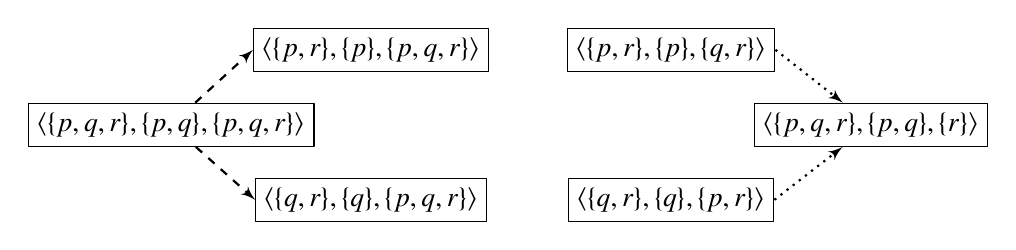
\begin{tikzpicture}[>=latex', join=bevel, initial text = , every node/.style=, scale=0.9]
  % States
  \node (tosplit) at (0bp, 0bp) [draw] {$\tuple{ \set{p,q,r} , \set{p,q} , \set{p,q,r} } $};

  \node (split1) at (80bp, 30bp) [draw] {$\tuple{ \set{p,r} , \set{p} , \set{p,q,r} } $};
  \node (split2) at (80bp, -30bp) [draw] {$\tuple{ \set{q,r} , \set{q} , \set{p,q,r} } $};


  \node (tomerge1) at (200bp, 30bp) [draw] {$\tuple{ \set{p,r} , \set{p} , \set{q,r} } $};
  \node (tomerge2) at (200bp, -30bp) [draw] {$\tuple{ \set{q,r} , \set{q} , \set{p,r} } $};
  \node (merged) at (280bp, 0bp) [draw] {$\tuple{ \set{p,q,r} , \set{p,q} , \set{r} } $};
  
  % Edges
  % \draw[->] (0) to node [above] {$-1$} (1);
  \draw[thick, dashed, ->] (tosplit) to node [] {} (split1.west);
  \draw[thick, dashed, ->] (tosplit) to node [] {} (split2.west);

  \draw[thick, dotted, ->] (tomerge1.east) to node [] {} (merged);
  \draw[thick, dotted, ->] (tomerge2.east) to node [] {} (merged);  
  
  % Selfloops
  % \draw (0) edge [loop above] node [above] {$+1$} (0);
\end{tikzpicture}

%% \begin{center} \fbox{ \xymatrix @C=1em { 
%% &*+<1pc>!<.5pc,-.5pc>[F]{\txt{ $\tuple{ \set{p,q,r} , \set{p,q} , \set{p,q,r} } $ }}
%% \ar[dl]{->}
%% \ar[dr]{->}
%% \\
%% *+<1pc>!<.5pc,-.5pc>[F]{\txt{ $\tuple{ \set{p,r} , \set{p} , \set{p,q,r} } $ }} 
%% 						&& *+<1pc>!<.5pc,-.5pc>[F]{\txt{ $\tuple{ \set{q,r} , \set{q} , \set{p,q,r} } $ }} 
%% \\
%% *+<1pc>!<.5pc,-.5pc>[F]{\txt{ $\tuple{ \set{p,r} , \set{p} , \set{q,r} } $ }} 
%% \ar[dr]{->}
%% 						&& *+<1pc>!<.5pc,-.5pc>[F]{\txt{ $\tuple{ \set{q,r} , \set{q} , \set{p,r} } $ }} 
%% 						  \ar[ld]{->}
%% \\
%% &*+<1pc>!<.5pc,-.5pc>[F]{\txt{ $\tuple{ \set{p,q,r} , \set{p,q} , \set{r} } $ }}
%% } } \end{center}
\caption{Examples of split and merge operations:
the left side illustrates the split of the model $\tuple{ \set{p,q,r} , \set{p,q} , \set{p,q,r} } $ into 
$\tuple{ \set{p,r} , \set{p} , \set{p,q,r} } $ and 
$\tuple{ \set{q,r} , \set{q} , \set{p,q,r} } $; 
the right side illustrates the merge of the models
$\tuple{ \set{p,r} , \set{p} , \set{p,q,r} } $ and 
$\tuple{ \set{q,r} , \set{q} , \set{p,q,r} } $ into
 $\tuple{ \set{p,q,r} , \set{p,q} , \set{r} } $.
}
\label{fig:splitmerge} 
\end{figure}
%\xymatrix @+1pc {
%& \underline{e} 
%     \ar@{->}@(ul,u)@[]^1
%     \ar@{->}[r]_{}^2
%                                & f
%				     \ar@{->}@(ur,u)@[]_{1,2} 
%				     						&
%        }


The set $\readset$ of readable variables of a model $\modl$ 
determines which models cannot be distinguished from $\modl$:
\begin{center}
$\modl \sim \modl'$ \ iff \ $\readset = \readset' , \writeset = \writeset' , \valuset \cap \readset = \valuset' \cap \readset' $.
\end{center}
Hence $\modl $ and $\modl'$ are indistinguishable if 
(1) they have the same readable and writable variables and  
(2) the valuations are identical as far as their readable parts are concerned.
%
This relation will serve to interpret tests: 
the test $\phi \testendo $ of a formula $\phi$ is conditioned by its truth in all read-indistinguishable models, i.e., 
in all models where the readable variables have the same truth value. 
%Clearly, $\modl \sim \modl'$ \ iff \ $\readset' = \readset$, $\writeset' = \writeset$, and there are $\valuset^+, \valuset^- \subseteq \propset \setminus \readset$ such that $\valuset' = (\valuset \setminus \valuset^-) \cup \valuset^+$. 


%----------------------------------------------------------%
\section{Language}\label{sec:language}
%----------------------------------------------------------%

Formulas and programs are defined by the following grammar,
where $p$ ranges over the set of propositional variables $\propset$:
%quid de $\pi \& \pi$ ou $\pi \sqcap \pi$ a la place de $\pi \pll \pi$ ?
\begin{align*}
\phi & ::= p \mid \top  \mid  \lnot \phi  \mid  \phi \lor \phi  \mid  \ldia \pi \phi ,
\\
\pi & ::= \assgntopV p \mid \assgnbotV p \mid
		\assgntopR p \mid \assgnbotR p \mid
		\assgntopW p \mid \assgnbotW p \mid
			%(\assgn \atm \phi) 
			\phi \testpdl \mid 
			\phi \testendo \mid 
			\pi ; \pi \mid \pi \ndet \pi \mid 
			\pi^\ast \mid \pi \pll \pi .
\end{align*}

The program $\assgntopV p$ makes $p$ true and $\assgnbotV p $ makes $p$ false. 
The executability of these two programs is conditioned by the writability of $p$. 
%
The program $\assgntopR p$ makes $p$ readable and 
$\assgnbotR p $ makes $p$ unreadable; similarly,
$\assgntopW p$ makes $p$ writable and 
$\assgnbotW p$ makes $p$ non-writable.
We suppose that these four programs are always executable. 
The program $\phi \testpdl$ is the PDL test that $\phi$, that we call \emph{exogenous};
$\phi \testendo $ is the \emph{endogenous} test that $\phi$: it is 
conditioned by the readability of the relevant variables of $\phi$. 

The formula $\lbox \pi \phi$ abbreviates $\lnot \ldia \pi \lnot \phi$.
Given an integer $n \geq 0$, the program $\pi^n$ is defined inductively by 
$\pi^0 = \top \testpdl $ and 
$\pi^{n+1} = \pi ; \pi^n $. 
Similarly, $\pi^{\leq n}$ is defined by 
$\pi^{\leq 0} = \top \testpdl $ and 
$\pi^{\leq n+1} = \top \testpdl \ndet (\pi ; \pi^{\leq n}) $. 
%The program $\ifthen{\phi}{\pi}$ abbreviates $(\phi \testpdl ; \pi) \ndet \lnot \phi \testpdl $.
%The program $\assgn \atm \phi$ abbreviates $(\phi \testpdl ; \assgntopV \atm) \ndet (\lnot \phi \testpdl ; \assgntopV \atm) $.
%\ah{elimine }
For a finite set of variables 
$P = \{p_i\}_{1 \leq  i \leq n}$ 
%$P = \{p_1,\ldots,p_n\}$ 
and associated programs 
$\{ \pi_i(p_i)\}_{1 \leq  i \leq n}$,
%$\{ \pi_1(p_1) , \ldots , \pi_n(p_n) \}$, 
we use the notation
$\seqseq{p \in P} \pi(p)$ to denote the sequence
$ \pi_1(p_1) ; \cdots ; \pi_n(p_n)$, in some order. 
We will make use of this notation with care to guarantee that the ordering of the elements of $P$ does not matter. 

The set of propositional variables occurring in a formula $\phi$ 
is noted $\propsetOf \phi $ and 
the set of those occurring in a program $\pi$ is noted $\propsetOf \pi $. 
For example, $\propsetOf{ p \lor \ldia{\assgntopV{q} } \lnot r } = \{p,q,r\}$. 


%----------------------------------------------------------%
\section{Semantics}\label{sec:interpretation} 
%----------------------------------------------------------%

%----------------------------------------------------------%
%\subsection{Interpretation of formulas and programs}

Let $\modl = \tuple{\readset,\writeset,\valuset}$ be a model. 
Formulas are interpreted as sets of models: 
\begin{center}\begin{tabular}{lll}
$\modl \models \top$
\\
$\modl \models p $ & iff & $p \in \valuset, \text{ for } p \in \propset$
\\
%$\modl \models \writable{p} $ & iff & $p \in \writeset$
%\\
%$\modl \models \readable p $ & iff & $p \in \readset$
%\\
$\modl \models \lnot \phi $ & iff & $\modl \not \models \phi $ 
\\
$\modl \models \phi \lor \psi$ & iff & $\modl \models \phi $ or $\modl \models \psi$ 
\\
$\modl \models \ldia \pi \phi $ & iff & there is a model $\modl'$ such that $\modl \intPgm{ \pi } \modl' $ and $\modl' \models \phi$
\end{tabular}\end{center}
Programs are interpreted as relations on the set of models: 
\begin{center}\begin{tabular}{lll}
$\modl \intPgm{ \assgntopV{p} } \modl'$ & iff & $\readset' = \readset$, $\writeset' = \writeset $, $\valuset' = \valuset \cup \{p\} $, and $p \in \writeset$
\\
$\modl \intPgm{ \assgnbotV{p} } \modl'$ & iff & $\readset' = \readset$, $\writeset' = \writeset $, $\valuset' = \valuset \setminus \{p\} $, and $p \in \writeset$
\\
$\modl \intPgm{ \assgntopR{p} } \modl'$ & iff & $\readset' = \readset \cup \{p\} $, $\writeset' = \writeset $, and $\valuset'= \valuset$
\\
$\modl \intPgm{ \assgnbotR{p} } \modl'$ & iff & $\readset' = \readset \setminus \{p\} $, $\writeset' = \writeset \setminus \{p\}$, and $\valuset'= \valuset$
\\
$\modl \intPgm{ \assgntopW{p} } \modl'$ & iff & $\readset' = \readset \cup \{p\} $, $\writeset' = \writeset \cup \{p\} $, and $\valuset' = \valuset$ 
\\
$\modl \intPgm{ \assgnbotW{p} } \modl'$ & iff & $\readset' = \readset$, $\writeset' = \writeset  \setminus \{p\} $, and $\valuset' = \valuset$ 
\\
$\modl \intPgm{ \phi \testpdl }\modl'$ & iff & $\modl = \modl'$ and $\modl \models \phi$ 
\\
$\modl \intPgm{ \phi \testendo }\modl'$ & iff & $\modl = \modl'$ and $\modl'' \models \phi$ for every $\modl''$ such that $\modl'' \sim \modl$
%``$\modl \intPgm{ \phi \testpdl } \modl'$ iff $\modl \sim \modl'$ and $\modl' \models \phi$''
%serait plus jolie, avec l'axiome de reduction
%$\ldia{\phi \testpdl } \psi \leqv \ \ldia{ \mathit{varyIfNotreadable}(\propsetOf \psi ) } (\phi \land \psi )$. 
%Mais plus difficile a justifer. 
\\
$\modl \intPgm{ \pi_1 ; \pi_2 } \modl'$ & iff & there is an $\modl''$ such that $\modl \intPgm{ \pi_1 } \modl''$ and 
												$\modl'' \intPgm{ \pi_2 } \modl'$
\\
$\modl \intPgm{ \pi_1 \ndet \pi_2 } \modl'$ & iff & $\modl \intPgm{ \pi_1 } \modl'$ or $\modl \intPgm{ \pi_2 } \modl'$ 
\\
$\modl \intPgm{ \pi^\ast } \modl'$ & iff & there is an $n \geq 0 $ such that $\modl \intPgm{ \pi } ^n \modl'$ 
\\
$\modl \intPgm{ \pi_1 \pll \pi_2 } \modl'$ & iff & there are $\modl_1, \modl_2, \modl'_1, \modl'_2$ such that %\\&&
$\splt{\modl}{\modl_1} {\modl_2} $, $\mrg{\modl'}{\modl'_1} {\modl'_2} $, \\&&
$\modl_1 \intPgm{ \pi_1 } \modl'_1$, 
$\readset_1 = \readset'_1 $, $\writeset_1 = \writeset'_1 $, $\valuset_1 \setminus \writeset_1 = \valuset'_1 \setminus \writeset'_1 , $ \\&&
$\modl_2 \intPgm{ \pi_2 } \modl'_2$, 
$\readset_2 = \readset'_2 $, $\writeset_2 = \writeset'_2 $, $\valuset_2 \setminus \writeset_2 = \valuset'_2 \setminus \writeset'_2 $ 
\end{tabular}\end{center}
In the interpretation of assignments of atomic formulas we require 
propositional variables to be modifiable, while 
readability and writability can be modified unconditionally.
When a variable is made writable then it is made readable, too, 
in order to guarantee the inclusion constraint on models; 
similarly when a variable is made unreadable. 
%
The interpretation of parallel composition $\pi_1 \pll \pi_2$ is such that both $\pi_1$ and $\pi_2$ only modify `their' variables: 
parallel composition $\pi_1 \pll \pi_2$ of two programs $\pi_1$ and $\pi_2$ 
relates two models $\modl$ and $\modl'$ when the following conditions are satisfied:
(1)~$\modl$ can be split into $\modl_1$ and $\modl_2$; 
(2)~the execution of $\pi_1$ on $\modl_1$ may lead to $\modl_1'$ and 
    the execution of $\pi_2$ on $\modl_2$ may lead to $\modl_2'$;
(3)~$\modl_1'$ and $\modl_2'$ can be merged into $\modl'$. 
Moreover, 
(4) the modifications are legal: $\pi_1$ and $\pi_2$ neither change readability nor writability, and 
each of them only modifies variables that were allocated to it by the split. 

Figure \ref{fig:ex:parallel} illustrates the interpretation of the parallel program $\assgnbotV p \pll \assgnbotV q$. 
Some more examples follow. 

\begin{figure}[t]
  \centering
  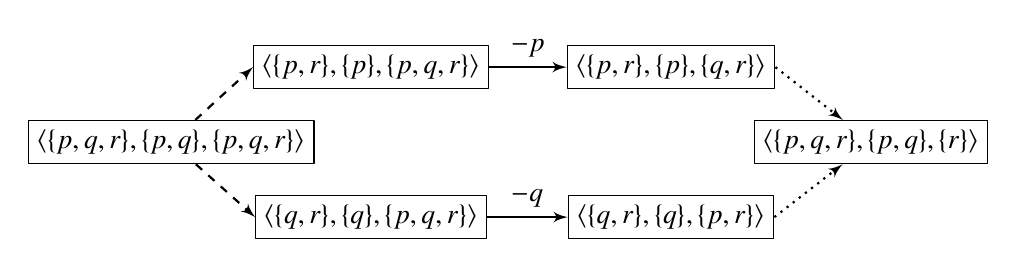
\begin{tikzpicture}[>=latex', join=bevel, initial text = , every node/.style=, scale=0.9]
  % States
  \node (tosplit) at (0bp, 0bp) [draw] {$\tuple{ \set{p,q,r} , \set{p,q} , \set{p,q,r} } $};

  \node (split1) at (80bp, 30bp) [draw] {$\tuple{ \set{p,r} , \set{p} , \set{p,q,r} } $};
  \node (split2) at (80bp, -30bp) [draw] {$\tuple{ \set{q,r} , \set{q} , \set{p,q,r} } $};


  \node (tomerge1) at (200bp, 30bp) [draw] {$\tuple{ \set{p,r} , \set{p} , \set{q,r} } $};
  \node (tomerge2) at (200bp, -30bp) [draw] {$\tuple{ \set{q,r} , \set{q} , \set{p,r} } $};
  \node (merged) at (280bp, 0bp) [draw] {$\tuple{ \set{p,q,r} , \set{p,q} , \set{r} } $};
  
  % Edges
  % \draw[->] (0) to node [above] {$-1$} (1);
  \draw[thick, dashed, ->] (tosplit) to node [] {} (split1.west);
  \draw[thick, dashed, ->] (tosplit) to node [] {} (split2.west);

  \draw[thick, ->] (split1) to node [above] {$\assgnbotV p$} (tomerge1);
  \draw[thick, ->] (split2) to node [above] {$\assgnbotV q$} (tomerge2);
  
  \draw[thick, dotted, ->] (tomerge1.east) to node [] {} (merged);
  \draw[thick, dotted, ->] (tomerge2.east) to node [] {} (merged);  
 
  
  % Selfloops
  % \draw (0) edge [loop above] node [above] {$+1$} (0);
\end{tikzpicture}

%% \begin{center} \fbox{ \xymatrix @C=1em { 
%% &*+<1pc>!<.5pc,-.5pc>[F]{\txt{ $\tuple{ \set{p,q,r} , \set{p,q} , \set{p,q,r} } $ }} 
%% \ar[dl]{->}
%% \ar[dr]{->}
%% \\
%% *+<1pc>!<.5pc,-.5pc>[F]{\txt{ $\tuple{ \set{p,r} , \set{p} , \set{p,q,r} } $ }} 
%% \ar[d]_{\assgnbotV p}{->}
%% 						&& *+<1pc>!<.5pc,-.5pc>[F]{\txt{ $\tuple{ \set{q,r} , \set{q} , \set{p,q,r} } $ }} 
%% 						  \ar[d]_{\assgnbotV q}{->}
%% \\
%% *+<1pc>!<.5pc,-.5pc>[F]{\txt{ $\tuple{ \set{p,r} , \set{p} , \set{q,r} } $ }} 
%% \ar[dr]{->}
%% 						&& *+<1pc>!<.5pc,-.5pc>[F]{\txt{ $\tuple{ \set{q,r} , \set{q} , \set{p,r} } $ }} 
%% 						  \ar[ld]{->}
%% \\
%% &*+<1pc>!<.5pc,-.5pc>[F]{\txt{ $\tuple{ \set{p,q,r} , \set{p,q} , \set{r} } $ }}
%% } } \end{center}
\caption{Illustration of an execution of $\assgnbotV p \pll \assgnbotV q$ at the model $\tuple{ \set{p,q,r} , \set{p,q} , \set{p,q,r} } $. 
}
\label{fig:ex:parallel} 
\end{figure}

\begin{example}
Suppose  
$\modl = \tuple{\readset,\writeset,\valuset}$ with $\writeset = \readset = \valuset = \{ p, q, r \}$. Then
$\modl' = \tuple{\readset,\writeset,\valuset'}$ with $\valuset' = \{ p, r\}$ is the only model such that 
$\modl \intPgm{  \assgntopV{p} \pll \assgnbotV{q} } \modl' $. 
\end{example}

The next example illustrates the last condition in the interpretation of parallel composition.

\begin{example}
The programs 
$\assgntopV p \pll \assgntopV p $ and
$\assgntopV p \pll (\assgntopW p ; \assgnbotV p ; \assgnbotR p ) $
cannot be executed on the model $\modl = \tuple{ \{p\}, \{p\}, \{p\} }$. 
%such that $\writeset = \valuset = \{p\}$. there is no $\modl'$ such that 
%$\modl \intPgm{ \assgntopV p \pll (\assgntopW p ; \assgnbotV p ; \assgnbotW p ) } \modl' $.
For the second, suppose there are $\modl_1$ and $\modl_2$ such that $\splt{\modl}{\modl_1} {\modl_2}$ and 
suppose $\assgntopV p$ is executed on $\modl_1$ and 
$\assgntopW p ; \assgnbotV p ; \assgnbotR p$ on $\modl_2$.
For $\assgntopV p$ to be executable we must have $p \in \writeset_1$, and therefore
$p \notin \writeset_2$ (and a fortiori $p \notin \readset_2$) because of the RW-disjointness condition. 
So $\modl_1 = \tuple{ \{p\}, \{p\}, \{p\} }$ and $\modl_2 = \tuple{ \emptyset, \emptyset, \{p\} }$.
Then 
$\modl_1' = \modl_1$ is the only model such that $\modl_1 \intPgm{ \assgntopV p } \modl_1' $; and 
$\modl_2' = \tuple{ \emptyset, \emptyset, \emptyset }$ is the only model such that $\modl_2 \intPgm{ \assgntopW p ; \assgnbotV p ; \assgnbotR p } \modl_2' $.
These two models cannot be merged because 
%the condition that in the interpretation of parallel composition that  
$\valuset_2' \setminus \writeset_2' % = \valuset_2' \setminus \writeset_2 
= \emptyset$ 
fails to be equal to 
$\valuset_2 \setminus \writeset_2 = \{p\}$. 
%
However, $\assgntopV p \pll ( \assgntopW p ; \assgntopV p ; \assgnbotR p )$
is executable on $\modl$: we have
$\splt{\modl}{\modl}{\tuple{\emptyset,\emptyset,\{p\}}}$ and 
$\modl \intPgm{\assgntopV p} \tuple{\{p\},\{p\},\{p\}}$ and
$\tuple{\emptyset,\emptyset,\{p\}} \intPgm{ \assgntopW p ; \assgntopV p ; \assgnbotR p } \tuple{\emptyset,\emptyset,\{p\} } $ and
$\mrg
{ \tuple{\{p\},\{p\},\{p\}} }
{ \tuple{\emptyset,\emptyset,\{p\}} }
{ \tuple{\{p\},\{p\},\{p\}} }$.
\end{example}

Let us finally illustrate the different semantics of the two test operators of our logic.
%PDL tests $\phi \testpdl$ do not depend on the readability of the variables that are tested and may be called \emph{exogeneous}. 
%Endogeneous tests $\phi \testendo$ also check the readability of the variables of $\phi$.

\begin{example}
Suppose $\modl$ is such that $p \notin \readset$ and $p \in \valuset$. 
Then the program $p \testpdl$ is executable on $\modl$ because $p \in \valuset$.
In contrast, there is no $\modl'$ such that $\modl \intPgm{ p \testendo } \modl'$, 
the reason being that there is always an $\modl''$ such that $\modl \sim \modl''$ and $p \notin \valuset''$,
hence $p \testendo$ is inexecutable. %at $\modl$. 
\end{example}

In practice, parallel programs should only contain endogenous tests in order to avoid that a subprogram accesses the truth value of a variable that is not among its readable variables.
Actually we have kept PDL tests for technical reasons only:
we could not formulate some of the reduction axioms without them. 

Satisfiability and validity of formulas are defined in the expected way.

\begin{example}
The formulas 
$\phi \limp \lbox{ \top \testendo \pll \top \testendo } \phi$, 
$\lbox{ \assgntopV p \pll \assgnbotV p } \bot$,
$\lbox{ \assgntopV p \pll \assgntopV p } \bot$ and 
$\lbox{ p \testendo \pll \assgntopV p } \bot$ 
whose programs were mentioned in the introduction are all valid. 
\end{example}

The formulas $\ldia{ \assgntopV p } \top $ and $\ldia{ \assgnbotV p } \top $ both express that $p$ is writable. 
Moreover, $\ldia{ p \testendo} \top $ expresses that $p$ is true and readable, and 
$\ldia{ \lnot p \testendo} \top $ expresses that $p$ is false and readable;
therefore $\ldia{ p \testendo} \top \lor \ldia{ \lnot p \testendo} \top $ 
%the nondeterministic composition $\ldia{ p \testendo \ndet \lnot p \testendo} \top $ 
expresses that $p$ is readable. 
This will be instrumental in our axiomatisation. 

Finally, for any model $\modl = \tuple{\readset, \writeset, \valuset}$ and $P \subseteq \propset$, we write
$\modl \modinter P$ for the model $\tuple{\readset \cap P, \writeset \cap P, \valuset \cap P}$.
This notation along with the following standard lemma
will be used several times in the remainder of this work.
%The next result says that the interpretation of formulas and programs is not sensitive to the values of propositional variables that do not occur in them, where `values' not only refers to the truth value but also to the readability and writability value. 

\begin{lemma}\label{theo:irrelevantVariables}
Let $\phi$ be a formula such that $\propsetOf \phi \cap P = \emptyset$ and
let $ \pi$ be a program such that $\propsetOf \pi \cap P = \emptyset$. Then the following hold:
\begin{enumerate}
\item\label{item:addValuationFormula}
$\tuple{\readset,\writeset,\valuset} \models \phi $ iff
$\tuple{\readset,\writeset,\valuset\cup P} \models \phi$;
\item\label{item:addAllFormula}
$\tuple{\readset,\writeset,\valuset} \models \phi $ iff
$\tuple{\readset\cup P,\writeset\cup P,\valuset} \models \phi$;
\item\label{item:addValuationProgram}
$\tuple{\readset,\writeset,\valuset} \intPgm \pi \tuple{\readset',\writeset',\valuset'} $ iff
$\tuple{\readset,\writeset,\valuset\cup P} \intPgm \pi \tuple{\readset',\writeset',\valuset'\cup P} $;
\item\label{item:addAllProgram}
$\tuple{\readset,\writeset,\valuset} \intPgm \pi \tuple{\readset',\writeset',\valuset'} $ iff
$\tuple{\readset\cup P,\writeset\cup P,\valuset} \intPgm \pi \tuple{\readset'\cup P,\writeset'\cup P,\valuset'} $;
\item\label{item:subAllProgram}
$\tuple{\readset,\writeset,\valuset} \intPgm \pi \tuple{\readset',\writeset',\valuset'} $ iff
$\tuple{\readset\setminus P,\writeset\setminus P,\valuset\setminus P} \intPgm \pi \tuple{\readset'\setminus P,\writeset'\setminus P,\valuset'\setminus P} $.
\end{enumerate}
\end{lemma}
\begin{proof}[sketch]
\ref{item:addValuationFormula} and \ref{item:addValuationProgram} are proved by simultaneous
induction on the size of $\phi$ and $\pi$.
\ref{item:addAllFormula} and \ref{item:addAllProgram} are proved similarly.
\ref{item:subAllProgram} is proved from \ref{item:addAllProgram} by instantiating $\readset$,
$\writeset$, $\valuset$, $\readset'$, $\writeset'$ and $\valuset'$ with respectively
$\readset\setminus P$, $\writeset\setminus P$, $\valuset\setminus P$, $\readset'\setminus P$,
$\writeset'\setminus P$ and $\valuset'\setminus P$.
\end{proof}



%----------------------------------------------------------%
\section{Axiomatisation via Reduction Axioms}\label{sec:axiomatisation}
%----------------------------------------------------------%

We axiomatise the validities of our logic by means of reduction axioms, as customary in dynamic epistemic logics \cite{DitmarschHoekKooi07}. 
These axioms transform every formula into a boolean combination of propositional variables
and formulas of the form
$\ldia{ \assgntopV p } \top $ and 
$\ldia{ p \testendo} \top \lor \ldia{ \lnot p \testendo} \top $. 
The former expresses that $p$ is writable: we abbreviate it by $\writable{p}$;
the latter expresses that $p$ is readable: we abbreviate it by $\readable p$. 
So we have:
\begin{align*}
\writable{p} &\eqdef \ldia{ \assgntopV p } \top 
\\
\readable p &\eqdef \ldia{ p \testendo} \top \lor \ldia{ \lnot p \testendo} \top 
\end{align*}

We start by eliminating all the program operators from formulas, where 
the elimination of parallel composition is done by sequentialising it while keeping track of the values of the atoms. 
After that step, the only remaining program operators 
either occur in formulas of the form $\readable p$ or $\writable p$, 
or are assignments of the form
$\ldia{ \assgntopV p} $,
$\ldia{ \assgnbotV p} $,
$\ldia{ \assgntopR p} $,
$\ldia{ \assgnbotR p} $,
$\ldia{ \assgntopW p} $, or
$\ldia{ \assgnbotW p} $. 
The assignments can be distributed over the boolean operators, taking advantage of the fact that all of them are deterministic modal operators 
(validating the Alt$_1$ axiom $\ldia \pi \phi \limp \lbox \pi \phi$). 
Finally, sequences of such modalities facing a propositional variable can be transformed into 
boolean combinations of readability and writability statements $\readable p$ and $\writable p$.
% of the form 
%$\ldia{ \assgntopV p } \top $, 
%$\ldia{ \assgnbotV p } \top $, 
%$\ldia{ p \testendo} \top$, and 
%$\ldia{ \lnot p \testendo} \top $. 
The only logical link between these statements is that 
%$\ldia{ \assgntopV p } \top $ and $\ldia{ \assgnbotV p } \top $ are equivalent and that 
writability of $p$ implies readability of $p$. 
This is captured by the axiom schema 
%$\ldia{ \assgntopV p } \top \leqv \ldia{ \assgnbotV p } \top $ and the latter by
$\writable p \limp \readable p$.
%$\ldia{ \assgntopV p } \top \limp \big( \ldia{ p \testendo} \top \lor \ldia{ \lnot p \testendo} \top \big) $. 

The sequentialisation of parallel composition uses copies of variables, so we start by introducing that notion. 
We then define some programs and formulas 
that will allow us to formulate the reduction axioms more concisely. 

%----------------------------------------------------------%
\subsection{Copies of Atomic Propositions}\label{sec:copyVars}

We are going to need fresh copies of each propositional variable, one per occurrence of the parallel composition operator. 
With parallel compositions based on separation, each concurrent program operates on its own model.
The introduced copies emulates this separation of models,
each concurrent program operating on a set of copies of propositional variables.

In order to keep things readable we neglect that the copies should be indexed by programs
and denote the copies of the variable $p$ by $\cp k p$, where $\mathbf{k}$ is some integer. 
In principle we should introduce a bijection between the indexes $\mathbf{k}$ and the subprogram they are attached to;
we however do not do so to avoid overly complicated notations.
%we formulate the sequentialisation of a parallel composition $\pi_1 \pll \pi_2$ by means of only two copies $\cp 1 p$ and $\cp 2 p$ of each variable $p$.

Given a set of propositional variables $P \subseteq \propset$ and an integer $\mathbf{k} \in \set{1,2}$, we define the set of copies
%$(p)$ xxxxxxxxxx
$\cp{k} P = \{ \cp{k} p \suchthat p \in P\}$. 
Similarly, we define copies of programs and formulas:
the program $\cp{k} \pi$ and the formula $\cp{k} \phi$ are obtained by replacing all their occurrences of
propositional variables $p$ by $\cp k p$. 

The following lemma will be instrumental in the soundness proof. 

\begin{lemma}\label{theo:copies}
Let $\pi$ be a program, 
let $\tuple{\readset,\writeset,\valuset}$ be a model, and 
let $\mathbf{k} \in \set{1,2}$. 
%If $\cp k p \notin \readset \cup \writeset \cup \valuset \cup \propsetOf \pi$ 
%for every $p \in \readset \cup \writeset \cup \valuset \cup \propsetOf \pi$ 
Then 
$$ \tuple{\readset,\writeset,\valuset} \intPgm{\pi} \tuple{\readset',\writeset',\valuset'} \text{ iff } 
\tuple{ \cp k {\readset},\cp k {\writeset},\cp k {\valuset}} \intPgm{\cp k \pi} \tuple{\cp k {\readset'},\cp k {\writeset'},\cp k {\valuset'}} . $$
\end{lemma}
\begin{proof}[sketch]
The proof relies on the fact that \DlpaPll satisfies the substitution rule.
The lemma can also be proved, like Lemma~\ref{theo:irrelevantVariables}, by simultaneous induction with the fact that
$\tuple{\readset, \writeset, \valuset} \models \phi$ if and only if
$\tuple{\cp k \readset, \cp k \writeset, \cp k \valuset} \models \cp k \phi$.
\end{proof}

Moreover, in order to force the semantics of the parallel composition operator, we associate to each copy $\cp k p$ two fresh variables $\cpr k p$ and $\cpw k p$,
denoting whether $\cp k p$ was respectively readable and writable just after the split.
We define $\storeset(P) =
\set{ \cpr k p \suchthat k \in \set{1,2}, p \in P} \cup
\set{ \cpw k p \suchthat k \in \set{1,2}, p \in P}$ as the set of all these fresh variables.


%----------------------------------------------------------%
\subsection{Useful Programs and formulas}\label{sec:usefulFml}

Let $P \subseteq \propset$ be some finite set of propositional variables. 
Table~\ref{fig:useful_programs} lists programs and formulas that will be useful to concisely formulate the reduction axioms.
%
Observe that the order of the variables in the sequential compositions $ \seqseq{p \in P} ( \cdots ) $ occurring in the above programs does not matter. 
Observe also that the only endogenous tests on the right hand side occur in readability statements $\readable p$. 
(Remember that $\readable p$ abbreviates $\ldia{ p \testendo} \top \lor \ldia{ \lnot p \testendo} \top $). 

\begin{table}[t]
\begin{align*}
\progsplit(P) =&\ \seqseq{p \in P} \Big(
  \assgntopW{\cp 1 p} ; \assgntopW{\cp 2 p} ;
\Big(
  \big( p \testpdl ; \assgntopV{ \cp{1}{p} } ; \assgntopV{ \cp{2}{p} } \big) \ndet 
  \big( \lnot p \testpdl ; \assgnbotV{ \cp{1}{p} } ; \assgnbotV{ \cp{2}{p} } \big) 
\Big) ; \assgnbotR{\cp 1 {p}} ; \assgnbotR{\cp 2 {p}} ;
\\& ~~~~~~~~~~~
\Big(
  \lnot \readable p  \testpdl \ndet
  \big(\writable{p} \testpdl ; ( \assgntopW{\cp 1 {p}} \ndet \assgntopW{\cp 2 {p}} ) \big) 			 \ndet
  \\& ~~~~~~~~~~~~~
  \big(\lnot \writable{p} {\land} \readable p  \testpdl ; \big( \assgntopR{\cp 1 {p}} \ndet \assgntopR{\cp 2 {p}} \ndet 
																			  (\assgntopR{\cp 1 {p}}  ; \assgntopR{\cp 2 {p}}) \big) \big) 
\Big)
\Big)
\\ %%%%%%%%%%%%%%%%%%%%%%%%%%%%%%%%%%%%%%%%%%%%%%%%%%%%
\progStore(P) =&\ \seqseq{p \in P} \seqseq{k \in \{1, 2\}} \Big(
  \assgntopW{\cpr k p} ; \assgntopW{\cpw k p} ;
\\& ~~~~~~~~~~~ 
  \big( \assgnpropV{\readable{\cp k p}}{\cpr k p} \big) ; \big( \assgnpropV{\writable{\cp k p}}{\cpw k p} \big)
\Big)
\\ %%%%%%%%%%%%%%%%%%%%%%%%%%%%%%%%%%%%%%%%%%%%%%%%%%%%
\progOkChange(P) =&\ \bigwedge_{p \in P} \bigwedge_{k \in \{1, 2\}} \Big(
( \cpr k p \leqv \readable{ \cp k {p} } ) 	\land 
( \cpw k p \leqv \writable{ \cp k {p} } ) 	\land 	
( \lnot \cpw k {p} \limp (p \leqv \cp k {p}) )
\Big)
\\ %%%%%%%%%%%%%%%%%%%%%%%%%%%%%%%%%%%%%%%%%%%%%%%%%%%%
\progmerge(P) =&\ \seqseq{p \in P} \Big(\big( 
\lnot \writable{p} \testpdl \ndet 
\\& ~~~~~~~~~~~ 
\big(	(\writable{ \cp{1}{p} } \land \cp{1}{p}) \lor 
		(\writable{ \cp{2}{p} } \land \cp{2}{p}) \testpdl ; \assgntopV p \big) \ndet 
\\& ~~~~~~~~~~~ 
\big(	(\writable{ \cp{1}{p} } \land \lnot \cp{1}{p}) \lor 
		(\writable{ \cp{2}{p} } \land \lnot \cp{2}{p}) \testpdl ; \assgnbotV p \big)
\big) ;
\\& ~~~~~~~~
\seqseq{k \in \{1, 2\}} \big(
  \assgnbotV{\cpr k p} ; \assgnbotV{\cpw k p} ; \assgntopW{\cp k p} ; \assgnbotV{\cp k p} ;
  \assgnbotR{\cpr k p} ; \assgnbotR{\cpw k p} ; \assgnbotR{\cp k p}
\big)
\Big)
\\ %%%%%%%%%%%%%%%%%%%%%%%%%%%%%%%%%%%%%%%%%%%%%%%%%%%%
\progFlatten(\pi_1, \pi_2) =&\ %
  \progsplit\left(\propsetOf{\pi_1 \pll \pi_2}\right) ;
  \progStore\left(\propsetOf{\pi_1 \pll \pi_2}\right) ;
%\\&\ %
  \cp 1 {\pi_1} ; \cp 2 {\pi_2} ;
%\\&\ %
  \progOkChange\left(\propsetOf{\pi_1 \pll \pi_2}\right) \testpdl ;
  \progmerge\left(\propsetOf{\pi_1 \pll \pi_2}\right)
\end{align*}
\caption{Useful programs, for all $P \subseteq \propset$ and all programs $\pi_1$ and $\pi_2$.
\label{fig:useful_programs}
}
\end{table}

The $\progsplit(P)$ program simulates the split operation by 
(1) assigning the truth value of every $p \in P$ to its copies $\cp 1 p$ and $\cp 2 p$ and
(2) nondeterministically assigning
two copies of each read and write variable in a way such that a counterpart of the RW-disjointness condition
$\writeset_1 \cap \readset_2 = \writeset_2 \cap \readset_1 = \emptyset$ is guaranteed.  
Note that the assignments $\assgntopW{ \cp{k}{p} }$ also make $\cp{k}{p} $ readable.
The following lemma formally states the main property of $\progsplit(P)$.
It can easily be proved by following the previous observations.

\begin{lemma}\label{lem:progsplit}
For all $P \subseteq \propset$, and all models $\modl$, $\modl_1$ and $\modl_2$ such that
$\modl \modinter P = \modl$,
$$ \splt \modl {\modl_1} {\modl_2} \text{ if and only if }
\modl \intPgm{\progsplit(P)} \modl'$$ with
$\readset' = \readset \cup \cp 1 {\readset_1} \cup \cp 2 {\readset_2}$,
$\writeset' = \writeset \cup \cp 1 {\writeset_1} \cup \cp 2 {\writeset_2}$, and
$\valuset' = \valuset \cup \cp 1 {\valuset_1} \cup \cp 2 {\valuset_2}$.
\end{lemma}

The $\progStore(P)$ program stores the readability and writability states of the
copies of the propositional variable into some fresh variables.
These variables are then used only in $\progOkChange(P)$.

The formula $\progOkChange(P)$ compares the current state with the state just after the split.
It is true if and only if
(1) readability values are identical, 
(2) writability values are identical, and
(3)~truth values are identical for non-writable variables.

The $\progmerge(P)$ program simulates the merge operation by reinstating all those 
read- and write-atoms that had been allocated to the first subprogram in the sequentialisation.
The following lemma formally states the main property of $\progmerge(P)$.
This lemma is weaker than Lemma~\ref{lem:progsplit} for $\progsplit(P)$.
The additional hypotheses are guaranteed to hold by the interplay of programs $\progsplit(P)$ and $\progStore(P)$,
and formula $\progOkChange(P)$.

\begin{lemma}\label{lem:progmerge}
For all models $\modl$, $\modl_1$ and $\modl_2$, all $P \subseteq \propset$ and all $\valuset^\sharp \subseteq P$,
such that $\modl \modinter P = \modl$,
        $\modl_1$ and $\modl_2$ are RW-disjoint,
        $\readset = \readset_1 \cup \readset_2$,
        $\writeset = \writeset_1 \cup \writeset_2$, and
        $\valuset_1 \setminus \writeset = \valuset_2 \setminus \writeset$,
$$\mrg \modl {\modl_1} {\modl_2} \text{ if and only if }
\modl' \intPgm{\progmerge(P)} \modl$$ with
$\readset' = \readset \cup \cp 1 {\readset_1} \cup \cp 2 {\readset_2} \cup \storeset(P)$,
$\writeset' = \writeset \cup \cp 1 {\writeset_1} \cup \cp 2 {\writeset_2} \cup \storeset(P)$, and
$\valuset' = \valuset^\sharp \cup \cp 1 {\valuset_1} \cup \cp 2 {\valuset_2}$
where $\valuset^\sharp$ is any subset of $P \cup \storeset(P)$ such that
$\valuset^\sharp \setminus \writeset = \valuset \setminus \writeset$.
\end{lemma}
\begin{proof}[sketch]
It suffices to prove that
$\modl' \intPgm{\progmerge(P)} \modl$ if and only if
$\valuset = (\valuset_1 \cap \writeset_1) \cup (\valuset_2 \cap \writeset_2) \cup (\valuset_1 \cap \valuset_2) $,
which is straightforward.
\end{proof}

Finally, the $\progFlatten(\pi_1, \pi_2)$ program emulates the execution of the program $\pi_1 \pll \pi_2$ as
a sequential composition of the previous programs.
Notice that there is no occurrence in $\progFlatten(\pi_1, \pi_2)$ of the parallel composition operator,
except inside $\pi_1$ and $\pi_2$.
Lemma~\ref{lem:pllequivalence} below states that the emulation is faithful.
We first need Lemma~\ref{lem:progClean},
which can be seen as an adaptation of lemma~\ref{theo:irrelevantVariables} to $\progFlatten(P)$.

\begin{lemma}\label{lem:progClean}
For all models $\modl$ and $\modl'$, and all programs $\pi_1$ and $\pi_2$,
$$
\modl \intPgm{\progFlatten(\pi_1,\pi_2)} \modl' \text{ iff }
(\modl \modinter \propsetOf{\pi_1 \pll \pi_2}) \intPgm{\progFlatten(\pi_1, \pi_2)} (\modl' \modinter \propsetOf{\pi_1 \pll \pi_2}).
$$
\end{lemma}
\begin{proof}[sketch]
It suffices to observe that all variables in $\propsetOf{\progFlatten(\pi_1, \pi_2)} \setminus \propsetOf{\pi_1 \pll \pi_2}$ are 
(1) made writable and initialized by $\progsplit$ or $\progStore$, and 
(2) set to false and made unreadable by $\progmerge$.
\end{proof}

Now our main lemma.

\begin{lemma}\label{lem:pllequivalence}
For all models $\modl$ and $\modl'$, and all programs $\pi_1$ and $\pi_2$,
$$
\modl \intPgm{\pi_1 \pll \pi_2} \modl' \text{ if and only if }
\modl \intPgm{\progFlatten(\pi_1, \pi_2)} \modl' \text{.}
$$
\end{lemma}
\begin{proof}[sketch]
Let $P = \propsetOf{\pi_1 \pll \pi_2}$. By Lemmas~\ref{theo:irrelevantVariables} and~\ref{lem:progClean},
we can assume that $\modl \modinter P = \modl$ and $\modl' \modinter P = \modl'$.

For the left-to-right direction, suppose there are models $\modl_1$, $\modl_2$, $\modl'_1$ and $\modl'_2$ such that
$\splt{\modl}{\modl_1} {\modl_2} $, $\mrg{\modl'}{\modl'_1} {\modl'_2} $,
$\modl_1 \intPgm{ \pi_1 } \modl'_1$, 
$\modl_2 \intPgm{ \pi_2 } \modl'_2$, 
$\readset_1 = \readset'_1 $, $\writeset_1 = \writeset'_1 $, $\valuset_1 \setminus \writeset_1 = \valuset'_1 \setminus \writeset'_1 , $
$\readset_2 = \readset'_2 $, $\writeset_2 = \writeset'_2 $, and $\valuset_2 \setminus \writeset_2 = \valuset'_2 \setminus \writeset'_2 $.
The following statements can be proved:
\begin{enumerate}
  \item\label{pllequivalence:ltr:split}
        $\modl \intPgm{\progsplit(P)} \modl^+_1$ with
        $\readset^+_1 = \readset \cup \cp 1 {\readset_1} \cup \cp 2 {\readset_2}$,
        $\writeset^+_1 = \writeset \cup \cp 1 {\writeset_1} \cup \cp 2 {\writeset_2}$, and
        $\valuset^+_1 = \valuset \cup \cp 1 {\valuset_1} \cup \cp 2 {\valuset_2}$.
        The proof relies on Lemma~\ref{lem:progsplit}.
  \item\label{pllequivalence:ltr:store}
        $\modl^+_1 \intPgm{\progStore(P)} \modl^+_2$ with
        $\readset^+_2 = \readset^+_1 \cup \storeset(P)$,
        $\writeset^+_2 = \writeset^+_1 \cup \storeset(P)$,
        $\valuset^+_2 = \valuset^+_1 \cup \valuset_{\storeset}$, and
        $\valuset_{\storeset} =
        \set{ \cpr k p \suchthat \cp k p \in \readset^+_1} \cup
        \set{ \cpw k p \suchthat \cp k p \in \writeset^+_1}$.
        Notice that
        $\valuset_{\storeset} =
        \set{ \cpr k p \suchthat p \in \readset_k} \cup
        \set{ \cpw k p \suchthat p \in \writeset_k}$.
  \item\label{pllequivalence:ltr:pi1}
        $\modl^+_2 \intPgm{\cp 1 {\pi_1}} \modl^+_3$ with
        $\readset^+_3 = \readset \cup \cp 1 {\readset'_1} \cup \cp 2 {\readset_2} \cup \storeset(P)$,
        $\writeset^+_3 = \writeset \cup \cp 1 {\writeset'_1} \cup \cp 2 {\writeset_2} \cup \storeset(P)$, and
        $\valuset^+_3 = \valuset \cup \cp 1 {\valuset'_1} \cup \cp 2 {\valuset_2} \cup \valuset_{\storeset}$.
        The proof relies on Lemmas~\ref{theo:irrelevantVariables} and~\ref{theo:copies}.
  \item\label{pllequivalence:ltr:pi2}
        $\modl^+_3 \intPgm{\cp 2 {\pi_2}} \modl^+_4$ with
        $\readset^+_4 = \readset \cup \cp 1 {\readset'_1} \cup \cp 2 {\readset'_2} \cup \storeset(P)$,
        $\writeset^+_4 = \writeset \cup \cp 1 {\writeset'_1} \cup \cp 2 {\writeset'_2} \cup \storeset(P)$, and
        $\valuset^+_4 = \valuset \cup \cp 1 {\valuset'_1} \cup \cp 2 {\valuset'_2} \cup \valuset_{\storeset}$.
  \item\label{pllequivalence:ltr:check}
        $\modl^+_4 \models \progOkChange(P)$.
  \item\label{pllequivalence:ltr:merge}
        $\modl^+_4 \intPgm{\progmerge(P)} \modl'$.
        The proof relies on Lemma~\ref{lem:progmerge}.
  \item $\modl \intPgm{\progFlatten(\pi_1, \pi2)} \modl'$.
\end{enumerate}

For the right-to-left direction, let us suppose that there are
models $\modl^+_1$, $\modl^+_2$, $\modl^+_3$ and $\modl^+_4$ such that
$\modl \intPgm{\progsplit(P)} \modl^+_1 \intPgm{\progStore(P)} \modl^+_2 \intPgm{\pi_1} \modl^+_3
\intPgm{\pi_2 ; \progOkChange(P)?} \modl^+_4 \intPgm{\progmerge(P)} \modl'$.
The following statements can be proved:
\begin{enumerate}
  \item\label{pllequivalence:rtl:split}
        $\splt{\modl}{\modl_1}{\modl_2}$ with
        $\readset_1 = \set{ p \suchthat \cp 1 p \in \readset^+_1}$,
        $\writeset_1 = \set{ p \suchthat \cp 1 p \in \writeset^+_1}$,
        $\valuset_1 = \set{ p \suchthat \cp 1 p \in \valuset^+_1}$,
        $\readset_2 = \set{ p \suchthat \cp 2 p \in \readset^+_1}$,
        $\writeset_2 = \set{ p \suchthat \cp 2 p \in \writeset^+_1}$, and
        $\valuset_2 = \set{ p \suchthat \cp 2 p \in \valuset^+_1}$.
        The proof relies on Lemma~\ref{lem:progsplit}.
  \item\label{pllequivalence:rtl:pi1}
        $\modl_1 \intPgm{\pi_1} \modl'_1$ with
        $\readset'_1 = \set{ p \suchthat \cp 1 p \in \readset^+_3}$,
        $\writeset'_1 = \set{ p \suchthat \cp 1 p \in \writeset^+_3}$, and
        $\valuset'_1 = \set{ p \suchthat \cp 1 p \in \valuset^+_3}$.
        The proof relies on Lemmas~\ref{theo:irrelevantVariables} and~\ref{theo:copies}.
  \item\label{pllequivalence:rtl:pi2}
        $\modl_2 \intPgm{\pi_2} \modl'_2$ with
        $\readset'_2 = \set{ p \suchthat \cp 2 p \in \readset^+_4}$,
        $\writeset'_2 = \set{ p \suchthat \cp 2 p \in \writeset^+_4}$, and
        $\valuset'_2 = \set{ p \suchthat \cp 2 p \in \valuset^+_4}$.
  \item\label{pllequivalence:rtl:check}
        $\readset_1 = \readset'_1 $, $\writeset_1 = \writeset'_1 $,
        $\valuset_1 \setminus \writeset_1 = \valuset'_1 \setminus \writeset'_1$,
        $\readset_2 = \readset'_2 $, $\writeset_2 = \writeset'_2 $, and
        $\valuset_2 \setminus \writeset_2 = \valuset'_2 \setminus \writeset'_2$.
        The proof relies on the fact that $\modl^+_4 \models \progOkChange(P)$, and
        $\valuset^+_4 \cap \storeset(P) =
        \set{ \cpr k p \suchthat p \in \readset_k} \cup
        \set{ \cpw k p \suchthat p \in \writeset_k}$.
  \item\label{pllequivalence:rtl:merge}
        $\mrg{\modl'}{\modl'_1}{\modl'_2}$.
        The proof relies on Lemma~\ref{lem:progmerge}.
  \item $\modl \intPgm{\pi_1 \pll \pi2} \modl'$.
\end{enumerate}
\end{proof}

%----------------------------------------------------------%
\subsection{Reduction Axioms for Program Operators}\label{sec:redax_pgmop} 

The reduction axioms for program operators are in Table~\ref{fig:redax_pgmops}.
Those for sequential and nondeterministic composition and for exogenous tests (PDL tests) are as in PDL. 
The one for endogenous tests $ \phi \testendo$ 
checks whether $\phi$ remains true for any possible value of the non-readable variables of $\phi$. 
That for the Kleene star is familiar from \Dlpa. 
That for parallel composition $\pi_1 \pll \pi_2$ executes $\pi_1$ and $\pi_2$ in sequence:
it starts by splitting up readability and writability between the two programs,
then executes $\pi_1$, checks whether $\pi_1$ didn't change the readability and writability variables
and whether all truth value changes it brought about are legal, 
and finally executes $\pi_2$ followed by the same checks for $\pi_2$.

\begin{table}[t]
\begin{align*}
\ldia{\phi \testpdl } \psi \leqv &\ \psi \land \phi
\\
\ldia{\phi \testendo } \psi \leqv &\ \psi \land \lbox{ ~ \seqseq{p \in \propsetOf \phi} \big(
\readable{p} \testpdl \ndet \big( \lnot \readable{p} \testpdl ; (\assgntopV{p} \ndet \assgnbotV{p}) \big) 
\big) } \phi
\\
\ldia{\pi_1 ; \pi_2}  \phi \leqv &\ \ldia{\pi_1 } \ldia{\pi_2}  \phi 
\\
\ldia{\pi_1 \ndet \pi_2}  \phi \leqv &\ \ldia{\pi_1 } \phi \lor \ldia{\pi_2}  \phi 
\\
\ldia{\pi^\ast}  \phi \leqv &\ \ldia{\pi^{\leq 2^{\card{\propsetOf{\phi}}}} }  \phi   
\\
\ldia{\pi_1 \pll \pi_2}  \phi \leqv &\ \ldia{ \progFlatten(\pi_1, \pi_2) } ~ \phi 
\end{align*}
\caption{Reduction axioms for program operators
\label{fig:redax_pgmops}
}
\end{table}

Observe that the validity of the reduction axiom for endogenous tests relies on the fact that the copies  
$\cp 1 p$ and $\cp 2 p$ that are introduced by the program 
$\progsplit( \propsetOf{\pi_1 \pll \pi_2} ) $ are fresh. 
%they neither occur in $\phi$ nor in $\pi_1$ nor in $\pi_2$. 
%
%Given a set of atomic formulas $X = \{\atm_1,\ldots,\atm_n\} $, 
%$\exists X \phi$ abbreviates 
%$$\ldia{ (\assgntopV{\atm_1} \ndet \assgnbotV{\atm_1}) ; \cdots ; (\assgntopV{\atm_n} \ndet \assgnbotV{\atm_n}) } \phi . $$
%Observe that the order of the variables does not matter. 
%
One may also note that the length of the right hand side can be shortened by restricting 
$\propsetOf{\pi_1 \pll \pi_2}$ to the propositional variables that are assigned by $\propsetOf{\pi_1 \pll \pi_2}$, i.e., 
to elements $p \in \propset$ such that $\assgntopV p$ or $\assgnbotV p$ occurs in $\propsetOf{\pi_1 \pll \pi_2}$.

The exhaustive application of the equivalences of Table~\ref{fig:redax_pgmops} from the left to the right 
results in formulas whose program operators are either endogenous tests occurring in a readability statement
$\readable p = \ldia{p \testendo} \top \lor \ldia{\lnot p \testendo} \top$, or 
assignments of the form
$\assgntopR p $, $\assgnbotR p $,
$\assgntopW p $, $\assgnbotW p $, 
$\assgntopV p $, or $\assgnbotV p $. 
%Remember that the last but one, $\assgntopV p $, can also be written as $\writable p$. 


%----------------------------------------------------------%
\subsection{Reduction Axioms for Boolean Operators}\label{sec:redax_atmpgm_bool} 

We now turn to modal operators $\ldia \pi$ where $\pi$ is an atomic assignment, i.e., $\pi$ is of the form 
$\assgntopR p $, $\assgnbotR p $,
$\assgntopW p $, $\assgnbotW p $, 
$\assgntopV p $, or $\assgnbotV p $. 
%(We will consider the special atomic formulas $\readable p$ in the next step.)
They are deterministic and can therefore be distributed over the boolean operators.
The corresponding reduction axioms are in Table~\ref{fig:redax_booleanops}.

\begin{table}[t]
\begin{align*}
\ldia{\assgntopV p} \top \leqv &\  \writable p
& \ldia{\assgnbotV p} \top \leqv &\  \writable p
\\
\ldia{\assgntopR p} \top \leqv &\ \top
& \ldia{\assgnbotR p} \top \leqv &\ \top
\\
\ldia{\assgntopW p} \top \leqv &\ \top
& \ldia{\assgnbotW p} \top \leqv &\ \top
%
\\
\ldia{\assgntopV p } \lnot \phi \leqv &\ 
					\writable{p} \land \lnot \ldia{\assgntopV p } \phi  
& \ldia{\assgnbotV p } \lnot \phi \leqv &\ 
					\writable{p} \land \lnot \ldia{\assgnbotV p } \phi 
\\
\ldia{\assgntopR p } \lnot \phi \leqv &\ 
					\lnot \ldia{\assgntopR p } \phi  
& \ldia{\assgnbotR p } \lnot \phi \leqv &\ 
					\lnot \ldia{\assgnbotR p } \phi 
\\
\ldia{\assgntopW p } \lnot \phi \leqv &\ 
					\lnot \ldia{\assgntopW p } \phi  
& \ldia{\assgnbotW p } \lnot \phi \leqv &\ 
					\lnot \ldia{\assgnbotW p } \phi 
%
\\
\ldia{\assgntopV p } (\phi \lor \psi) \leqv &\ \ldia{\assgntopV p } \phi \lor \ldia{\assgntopV p } \psi 
& \ldia{\assgnbotV p } (\phi \lor \psi) \leqv &\ \ldia{\assgnbotV p } \phi \lor \ldia{\assgnbotV p } \psi 
\\
\ldia{\assgntopR p } (\phi \lor \psi) \leqv &\ \ldia{\assgntopR p } \phi \lor \ldia{\assgntopR p } \psi 
& \ldia{\assgnbotR p } (\phi \lor \psi) \leqv &\ \ldia{\assgnbotR p } \phi \lor \ldia{\assgnbotR p } \psi 
\\
\ldia{\assgntopW p } (\phi \lor \psi) \leqv &\ \ldia{\assgntopW p } \phi \lor \ldia{\assgntopW p } \psi 
& \ldia{\assgnbotW p } (\phi \lor \psi) \leqv &\ \ldia{\assgnbotW p } \phi \lor \ldia{\assgnbotW p } \psi 
\end{align*}
\caption{Reduction axioms for boolean operators
\label{fig:redax_booleanops}
}
\end{table}

In the first equivalence $\ldia{\assgntopV p} \top \leqv \  \writable p$, 
the right hand side is nothing but an abbreviation of the left hand side. 
We nevertheless state it in order to highlight that the exhaustive application of these reduction axioms 
results in sequences of atomic assignments facing 
either $\writable p$ or $\readable q$. 
These sequences are going to be reduced in the next step. 


%----------------------------------------------------------%
\subsection{Reduction Axioms for Assignments}\label{sec:redax_atmpgm} 

\begin{table}[t]
\begin{align*}
\ldia{\assgntopV p } q \leqv &\ \begin{cases} 
					\writable{p} 	& \text{ if } q = p \\
					\writable{p} \land q & \text{ otherwise } 
					\end{cases} 
& \ldia{\assgnbotV p } q \leqv &\ \begin{cases} 
					\bot 	& \text{ if } q = p \\
					\writable{p} \land q & \text{ otherwise } 
					\end{cases} 
\\
\ldia{\assgntopR p } q \leqv &\ q
& \ldia{\assgnbotR p } q \leqv &\ q
\\
\ldia{\assgntopW p } q \leqv &\ q
& \ldia{\assgnbotW p } q \leqv &\ q
%
\\
\ldia{\assgntopV p} \readable q \leqv &\  \writable p \land \readable q
& \ldia{\assgnbotV p} \readable q \leqv &\  \writable p \land \readable q
\\
\ldia{\assgntopR p} \readable q \leqv &\ \begin{cases}
								\top & \text{ if } q = p \\
								\readable q & \text{ otherwise }
								\end{cases}
& \ldia{\assgnbotR p} \readable q \leqv &\ \begin{cases}
								\bot & \text{ if } q = p \\
								\readable q & \text{ otherwise }
								\end{cases}
\\
\ldia{\assgntopW p} \readable q \leqv &\ \begin{cases}
                \top & \text{ if } q = p \\
                \readable q & \text{ otherwise }
                \end{cases}
& \ldia{\assgnbotW p} \readable q \leqv &\ \readable q
%
\\
\ldia{\assgntopV p } \writable{q} \leqv &\ \writable{p} \land \writable{q}
& \ldia{\assgnbotV p } \writable{q} \leqv &\ \writable{p} \land \writable{q}
\\
\ldia{\assgntopR p } \writable{q} \leqv &\ \writable{q}
& \ldia{\assgnbotR p } \writable{q} \leqv &\ \begin{cases}
                \bot & \text{ if } q = p \\
                \writable{q} & \text{ otherwise } 
								\end{cases}
\\
\ldia{\assgntopW p } \writable{q} \leqv &\ \begin{cases}
								\top & \text{ if } q = p \\
								\writable{q} & \text{ otherwise }
								\end{cases}
& \ldia{\assgnbotW p } \writable{q} \leqv &\ \begin{cases}
								\bot & \text{ if } q = p \\
								\writable{q} & \text{ otherwise }
								\end{cases}
\end{align*}
\caption{Reduction axioms for assignments
\label{fig:redax_assignments}
}
\end{table}

When atomic programs face propositional variables or readability and writability statements 
then the modal operator can be eliminated (sometimes introducing a writability statement $\writable{p}$). 
The reduction axioms doing that are in Table~\ref{fig:redax_assignments}.

As announced, the exhaustive application of the above equivalences results in boolean combinations of 
propositional variables and readability and writability statements. 

%----------------------------------------------------------%
\subsection{Soundness, Completeness, and Decidability} 

Let us call \DlpaPll our extension of \Dlpa with parallel composition. 
Its axiomatisation is made up of 
\begin{itemize}
\item
an axiomatisation of propositional logic;
\item
the equivalences of Sections \ref{sec:redax_pgmop}, 
\ref{sec:redax_atmpgm_bool}, 
and \ref{sec:redax_atmpgm};
%\item
%the axiom about writability $\ldia{ \assgnbotV p } \top \leqv \writable p$, which abbreviates
%$\ldia{ \assgntopV p } \top \leqv \ldia{ \assgnbotV p } \top $;
\item
the inclusion axiom schema $\writable{p} \limp \readable p$, which is an abbreviation of the formula
$\ldia{ \assgntopV p } \top \limp \big( \ldia{ p \testendo} \top \lor \ldia{ \lnot p \testendo} \top \big) $;
\item
the rule of equivalence for the modal operator %$\text{RE} \big(\ldia \pi \Big)$ 
``from $\phi \leqv \psi$ infer $\ldia \pi \phi \leqv \ldia \pi \psi $''.
\end{itemize}

\begin{theorem}\label{theo:axiomatisationsound}
The axiomatisation of \DlpaPll is sound:
if $\phi$ is provable with the axiomatics of \DlpaPll then it is \DlpaPll valid.
\end{theorem}
\begin{proof}[sketch]
We have to show that the inference rules preserve validity and the axioms are valid. 
For the reduction axiom for endogenous test, it suffices to observe that
$\modl \intPgm{\assgntopV p \ndet \assgnbotV p} \modl'$ if and only if $\modl \sim \modl'$.
The proof of validity of the reduction axiom for Kleene star can easily be adapted from the one in~\cite{BalbianiHerzigTroquard-Lics13}.
The case of the reduction axiom for parallel composition is handled by Lemma~\ref{lem:pllequivalence}.
All other cases are straightforward.
\end{proof}

\begin{theorem}
The axiomatisation of \DlpaPll is complete:
if $\phi$ is \DlpaPll valid then it is provable in the axiomatics of \DlpaPll. 
\end{theorem}
\begin{proof}
The reduction axioms of Sections \ref{sec:redax_pgmop}, \ref{sec:redax_atmpgm_bool}, and \ref{sec:redax_atmpgm} 
allow us to transform any formula into an equivalent boolean combination of 
propositional variables and readability and writability statements. 
(Their application requires the rule of replacement of equivalents, which is derivable 
because we have rules of equivalence for all the connectives of the language, 
in particular the above $RE(\ldia \pi)$.)
Let $\phi$ be the resulting formula. 
Then $\phi$ has a \DlpaPll model if and only if 
$$\phi \land 
\bigwedge_{p \in \propset} \big( \writable{p} \limp \readable p \big) $$
%\land \bigwedge_{p \in \propset} \big( \ldia{ \assgnbotV p } \top \leqv \writable p \big) $$
has a model in propositional logic, where in propositional logic,
$\readable p$ and $\writable{p}$ are considered to be arbitrary propositional variables; so
there is a priori no connection between them nor with the propositional variable $p$. 
\end{proof}


Based on the reduction of \DlpaPll formulas to boolean formulas 
(and the transformation of $\readable p$ and $\writable{p}$ from abbreviations into propositional variables),
we may check the satisfiability of \DlpaPll formulas by means of propositional logic SAT solvers. 
This is however suboptimal because reduction may result in a formula that is super-exponentially longer than the original formula. 
In the next section we explore another route.


%----------------------------------------------------------%
\section{Complexity via Translation into \Dlpa}\label{sec:complexity}
%----------------------------------------------------------%

We establish PSPACE complexity of \DlpaPll satisfiability and model checking by translating formulas and programs to 
Dynamic Logic of Propositional Assignments \Dlpa. 
The language of the latter is the fragment of that of \DlpaPll:
it has neither endogenous tests, nor readability and writability assignments, nor parallel composition. 
So the language of \Dlpa is built by the following grammar: 
\begin{align*}
\phi & ::= p \mid \top \mid \lnot \phi \mid (\phi \lor \phi) \mid \ldia \pi \phi
\\
\pi & ::= \assgntopV p \mid \assgnbotV p \mid
		%\assgntopR p \mid \assgnbotR p \mid
		%\assgntopW p \mid \assgnbotW p \mid
			\phi \testpdl \mid 
			%\phi \testendo \mid 
			(\pi ; \pi) \mid (\pi \ndet \pi) \mid 
			\pi^\ast 
			%\mid (\pi \pll \pi)
\end{align*} 
None of the operators of the language refers to the $\readset$-component or the $\writeset$-component of models. 
The interpretation of \Dlpa formulas and programs therefore only requires a valuation $\valuset$. 
%instead of triples, models are just valuations.

Our translation from \DlpaPll to \Dlpa eliminates endogenous tests and parallel composition. 
This is done in a way that is similar to their reduction axioms of Table~\ref{fig:redax_pgmops}.
It moreover transforms readability and writability statements into special propositional variables $\readable p$ and $\writable p$, similar to the reduction axioms of Table~\ref{fig:redax_assignments}.
%into propositional logic formulas in Section \ref{sec:axiomatisation}. 

To make this formal, let the set of \emph{atomic formulas} be
$$ \atmset = \propset \cup \{ \writable{p} \suchthat p \in \propset \} \cup \{ \readable p \suchthat p \in \propset \} . $$
%where the intended meanings of the `write-variable' $\writable{p}$ and the `read-variable' $\readable p$ are respectively that $p$ can be modified and that $p$ can be read. 
%We use $p, q, p', p_1,\ldots$ for variables in $\propset$ and 
%$\atm, \atm', \atmb, \atm_1,\ldots$ for atomic formulas in $\atmset$. 
Given a set of propositional variables $P \subseteq \propset$, 
$\readOf P = \{ \readable p \suchthat p \in P \}$ 
is the associated set of read-variables and 
$\writeOf P = \{ \writable{p} \suchthat p \in P \}$ 
is the associated set of write-variables. 
So $\atmset = \propset \cup \readOf \propset \cup \writeOf \propset$. 
%
As before, the set of propositional variables occurring in a formula $\phi$ is noted $\propsetOf \phi $ and 
the set of those occurring in a program $\pi$ is noted $\propsetOf \pi $. %similarly for $\atmset(\phi)$ and $\atmset(\pi) 
This now includes the $p$'s in $\readable p$ and $\writable{p}$. 
For example, $\propsetOf{ p \land \ldia{\assgntopV{w_q} } \lnot \readable p } = \{p,q\}$. % and $\atmset( p \land w_{p'} ) = \{p , w_{p'}\}$. 

We translate the \DlpaPll programs
$\assgntopR{p}$, 
$\assgnbotR{p}$, 
$\assgntopW{p}$, and 
$\assgnbotW{p}$ 
into the \Dlpa programs 
$\assgntop{ \readable{p}}$,
$\assgnbot{ \readable{p}}$,
$\assgntop{ \writable{p}}$ and
$\assgnbot{ \writable{p}}$.
Moreover, we have to `spell out' that 
$\assgnbot{ \writable p }$ has side effect $\assgnbot{ \readable p }$ and that  
$\assgntop{ \readable p }$ has side effect $\assgntop{ \writable p }$. 
So the programs and formulas of Table~\ref{fig:useful_programs} become the following \Dlpa programs and formulas:
\begin{align*}
\progsplit(P) =&\ \seqseq{p \in P} \Big( 
\Big(
  \big( p \testpdl ; \assgntopV{ \cp{1}{p} } ; \assgntopV{ \cp{2}{p} } \big) \ndet 
  \big( \lnot p \testpdl ; \assgnbotV{ \cp{1}{p} } ; \assgnbotV{ \cp{2}{p} } \big) 
\Big) ;
\\& ~~~~~~~~~~~
\assgnbot{ \writable{\cp 1 {p}}} ; \assgnbot{ \readable{\cp 1 {p}}} ; \assgnbot{ \writable{\cp 2 {p}}} ; \assgnbot{ \readable{\cp 2 {p}}} ;
\\& ~~~~~~~~~~~
\Big(
  \lnot \readable p  \testpdl \ndet 
  \\& ~~~~~~~~~~~~~
  \big(\writable{p} \testpdl ; ( (\assgntop{ \readable{\cp 1 {p}}} ; \assgntop{ \writable{\cp 1 {p}}}) \ndet (\assgntop{ \readable{\cp 2 {p}}} ; \assgntop{ \writable{\cp 2 {p}}}) ) \big) 			 \ndet
  \\& ~~~~~~~~~~~~~
  \big(\lnot \writable{p} {\land} \readable p  \testpdl ; \big( \assgntop{ \readable{\cp 1 {p}}} \ndet \assgntop{ \readable{\cp 2 {p}}} \ndet 
(\assgntop{ \readable{\cp 1 {p}}}  ; \assgntop{ \readable{\cp 2 {p}}}) \big) \big) 
\Big)
\Big)
\displaybreak[0]
\\ %%%%%%%%%%%%%%%%%%%%%%%%%%%%%%%%%%%%%%%%%%%%%%%%%%%%%%%%%%%%%%%%%%%%%
\progStore(P) =&\ \seqseq{p \in P} \seqseq{k \in \{1, 2\}} \Big(
  \big( \assgnpropV{\readable{\cp k p}}{\cpr k p} \big) ;
  \\& ~~~~~~~~~~~~~
  \big( \assgnpropV{\writable{\cp k p}}{\cpw k p} \big)
\Big)
\displaybreak[0]
\\ %%%%%%%%%%%%%%%%%%%%%%%%%%%%%%%%%%%%%%%%%%%%%%%%%%%%%%%%%%%%%%%%%%%%%
\progOkChange(P) =&\ \bigwedge_{p \in P} \bigwedge_{k \in \{1, 2\}} \Big(
( \cpr k p \leqv \readable{ \cp k {p} } ) 	\land 
( \cpw k p \leqv \writable{ \cp k {p} } ) 	\land 	
( \lnot \cpw k {p} \limp (p \leqv \cp k {p}) )
\Big)
\displaybreak[0]
\\ %%%%%%%%%%%%%%%%%%%%%%%%%%%%%%%%%%%%%%%%%%%%%%%%%%%%%%%%%%%%%%%%%%%%%
\progmerge(P) =&\ \seqseq{p \in P} \Big(\big( 
\lnot \writable{p} \testpdl \ndet 
\\& ~~~~~~~~~~~ 
\big(	(\writable{ \cp{1}{p} } \land \cp{1}{p}) \lor 
		(\writable{ \cp{2}{p} } \land \cp{2}{p}) \testpdl ; \assgntopV p \big) \ndet 
\\& ~~~~~~~~~~~ 
\big(	(\writable{ \cp{1}{p} } \land \lnot \cp{1}{p}) \lor 
		(\writable{ \cp{2}{p} } \land \lnot \cp{2}{p}) \testpdl ; \assgnbotV p \big)
\big) ;
\\& ~~~~~~~~
\seqseq{k \in \{1, 2\}} \big(
  \assgnbotV{\cpr k p} ; \assgnbotV{\cpw k p} ; \assgnbotV{\cp k p} ;
  \assgnbotV{\writable{\cp k p}} ; \assgnbotV{\readable{\cp k p}}
\big)
\Big)
\displaybreak[0]
\\ %%%%%%%%%%%%%%%%%%%%%%%%%%%%%%%%%%%%%%%%%%%%%%%%%%%%%%%%%%%%%%%%%%%%%
\progFlatten(\pi_1, \pi_2) =&\ %
  \progsplit\left(\propsetOf{\pi_1 \pll \pi_2}\right) ;
  \progStore\left(\propsetOf{\pi_1 \pll \pi_2}\right) ;
%\\&\ %
  \cp 1 {\pi_1} ; \cp 2 {\pi_2} ;
%\\&\ %
  \progOkChange\left(\propsetOf{\pi_1 \pll \pi_2}\right) \testpdl ;
  \progmerge\left(\propsetOf{\pi_1 \pll \pi_2}\right)
\end{align*}
Notice that
readability and writability statements are no longer \DlpaPll abbreviations, but are now \Dlpa propositional variables. 

Given a \DlpaPll program or formula, its translation into \Dlpa basically follows the reduction axiom for endogenous tests $\testendo$ and parallel composition $ \pll $ of Table~\ref{fig:redax_pgmops}. 
We replace:
\begin{enumerate}
\item
all occurrences of $\phi \testendo $ with 
$\left[\seqseq{p \in \propsetOf \phi} \Big(
\readable{p} \testpdl \ndet \big( \lnot \readable{p} \testpdl ; (\assgntopV{p} \ndet \assgnbotV{p}) \big) 
\Big)\right] \phi \testpdl $,
\item
all occurrences of $ \pi_1 \pll \pi_2 $ with $\progFlatten(\pi_1, \pi_2)$,
\item
all occurrences of $\assgntopV p$ with $\writable p ? ; \assgntopV p$,
\item
all occurrences of $\assgnbotV p$ with $\writable p ? ; \assgnbotV p$,
\item
all occurrences of $\assgntopR{p}$ with $\assgntop{ \readable{p}}$,
\item
all occurrences of $\assgnbotR{p}$ with $\assgnbot{ \writable{p}} ; \assgnbot{ \readable{p}}$,
\item
all occurrences of $\assgntopW{p}$ with $\assgntop{ \readable{p}} ; \assgntop{ \writable{p}}$,
\item
all occurrences of $\assgnbotW{p}$ with $\assgnbot{ \writable{p}}$.
%$\assgnbot{ \writable p }$ with $\assgnbot{ \writable p } ; \assgnbot{ \readable p }$ and all occurrences of 
%$\assgntop{ \readable p }$ with $\assgntop{ \readable p } ; \assgntop{ \writable p }$, for $p \in \propset$.
\end{enumerate}
Let $t(\pi)$ be the translation of the \DlpaPll program $\pi$ and
$t(\phi)$ the translation of the \DlpaPll formula $\phi$.
Remember that when $t(\pi)$ and $t(\phi)$ are interpreted in \Dlpa, the variables $\readable p$ and $\writable{p}$ 
are considered to be arbitrary propositional variables. 

\begin{lemma}\label{lem:dlpatradcorrect}
For all \DlpaPll programs $\pi$ and formula $\phi$, and all \DlpaPll models $\modl$ and $\modl'$ such that $\modl \modinter P = \modl$,
\begin{align*}
  \modl \intPgm{\pi} \modl' &\text{ if and only if } \valuset^+ \intPgm{t(\pi)}^{\Dlpa} \valuset'^+ \text{, and} \\
  \modl \models \phi        &\text{ if and only if } \valuset^+ \models_{\Dlpa} t(\phi)
\end{align*}
where $\valuset^+  = \valuset  \cup \readOf{\readset } \cup \writeOf{\writeset }$
and   $\valuset'^+ = \valuset' \cup \readOf{\readset'} \cup \writeOf{\writeset'}$.
\end{lemma}
\begin{proof}[sketch]
The proof is by simultaneous induction on the size of $\pi$ or $\phi$.
The cases for endogenous tests and parallel compositions are similar to the ones in the proof of Theorem~\ref{theo:axiomatisationsound}.
The other cases are straightforward.
\end{proof}

The following theorem is a direct corollary of the previous lemma.

\begin{theorem}
A \DlpaPll formula $\phi$ is \DlpaPll-satisfiable if and only if the \Dlpa formula
$t(\phi) \land \bigwedge_{p \in \propsetOf \phi } (\writable{p} \limp \readable p)$ 
is \Dlpa satisfiable.
\end{theorem}

%The next result folows from the fact that the length of $t(\phi)$ is polynomial in the length of $\phi$. 
We can now state our complexity results.

\begin{lemma}\label{lem:polynomial}
The translation $t$ is polynomial.
\end{lemma}
\begin{proof}
It can easily be checked that for all $P$, $\progsplit(P)$, $\progStore(P)$, $\progOkChange(P)$ and $\progmerge(P)$ are linear in the size of $P$.
Therefore, $\progFlatten(\pi_1, \pi_2)$ is linear in the size of $\pi_1$ plus the size of $\pi_2$.
Similarly, 
$\left[\seqseq{p \in \propsetOf \phi} \Big(
\readable{p} \testpdl \ndet \big( \lnot \readable{p} \testpdl ; (\assgntopV{p} \ndet \assgnbotV{p}) \big) 
\Big)\right] \phi \testpdl $ is linear in the size of $\phi$.
All other translation expressions are clearly linear too.
Hence, by applying $t$ from the root of the syntax tree to its leaves, $t(\phi)$ can be computed in time polynomial in the size of $\phi$.
\end{proof}

\begin{theorem}
\DlpaPll model and satisfiability checking are both PSPACE complete.
\end{theorem}
\begin{proof}
Since any \Dlpa formula is a \DlpaPll formula, and \Dlpa model and satisfiability checking has been proved in~\cite{BalbianiHST14} to be PSPACE complete,
\DlpaPll model and satisfiability checking are PSPACE hard.
By Lemmas~\ref{lem:dlpatradcorrect} and~\ref{lem:polynomial}, \DlpaPll model and satisfiability checking are also in PSPACE.
\end{proof}

%----------------------------------------------------------%
\section{Conclusion}\label{sec:conclusion}
%----------------------------------------------------------%

We have added to Dynamic Logic of Propositional Assignments \Dlpa
a parallel composition operator in the spirit of separation logics. 
To that end we have augmented \Dlpa valuations by readability and writability information. 
We have adopted a stricter stance on race conditions than in the approach of \cite{HerzigEtal-Ijcai19} 
where e.g.\ the program $\assgntop p \pll \assgntop p$ is executable.
We have provided a complete axiomatisation in terms of reduction axioms, 
ensuring at the same time decidability. 
We have also proved PSPACE complexity via a translation to \Dlpa. 

The mathematical properties of \DlpaPll compare favourably with 
the high complexity or even undecidability of the 
other extensions of dynamic logic by a separating parallel composition operator that were proposed in the literature
\cite{BalbianiT14,Boudou16}.
%DBLP:journals/logcom/BenevidesS14,
%DBLP:journals/tcs/Benevides17
Just as ours, the latter line of work is in the spirit of separation logic, having splitting and merging operations that are defined on system states. 
The axiomatisation that was introduced and studied in \cite{DBLP:journals/logcom/BalbianiB18} is restricted to the star-free fragment and the authors had to add propositional quantifiers in order to make parallel composition definable. 
This contrasts with the simplicity of our axiomatisation of \DlpaPll that we obtained by adding reduction axioms to the axiomatisation of \Dlpa. 
Just as \Dlpa can be viewed as an instance of PDL%
---the interpretation of atomic programs moves from PDL's abstract relation between states to concrete updates of valuations\mbox{---,}
\DlpaPll can be viewed as an instance of the logic of \cite{DBLP:journals/entcs/BenevidesFV11}
where the interpretation of parallel composition no longer resorts to
an abstract relation $\star$ associating three states, 
but instead has concrete functions that split and merge valuations and that are constrained by readability and writability information. 

%----------------------------------------------------------%
\section{Acknowledgements}
%----------------------------------------------------------%
The paper benefited from comments and remarks from the reviewers as well as from the attendees of DaL\'i 2019, 
in particular Alexandru Baltag, Raul Fervari, Rainer H\"ahnle and Dexter Kozen. 
We did our best take their comments into account. 


\appendix
\section{Associativity}
\newcommand{\modla}{\mathsf a}
\newcommand{\readseta}{\mathsf {Rda}}
\newcommand{\writeseta}{\mathsf {Wra}}
\newcommand{\valuseta}{\mathsf {Va}}

Alongside commutativity, associativity is a desirable property of a parallel composition operator. While the operator defined in Section~\ref{sec:interpretation} is clearly commutative, whether it is associative does not strike the eye. In fact, a detailed proof of it is rather cumbersome. We present it here.

\begin{proposition}\label{prop:associativity}
$\modl \intPgm{ \pi_1 \pll (\pi_2 \pll \pi_3) } \modl'$ iff $\modl \intPgm{ (\pi_1 \pll \pi_2) \pll \pi_3 } \modl'$.
\end{proposition}
\begin{proof}


  \begin{figure}[h]
    \centering
    \begin{tabular}{lcl}
      $\exists \modl_1, \modl_*, \modl_2, \modl_3, \modl'_1, \modl'_2, \modl'_3, \modl'_*$': &  ~~~~~\emph{iff}~~~~~&    $\exists \modla_\#, \modla_3, \modla_1, \modla_2, \modla_1', \modla_2', \modla_\#', \modla_3'$:\\
      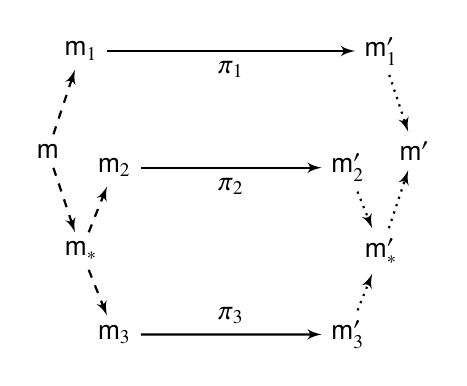
\begin{tikzpicture}[>=latex', join=bevel, initial text = , every node/.style=, scale=1.2]
  % States
  \node (m) at (0bp, 0bp) {$\modl$};

  \node (m1) at (10bp, 30bp) {$\modl_1$};
  \node (mast) at (10bp, -30bp) {$\modl_*$};

  \node (m1prime) at (100bp, 30bp) {$\modl'_1$};
  \node (m2) at (20bp, -5bp) {$\modl_2$};  
  \node (m3) at (20bp, -55bp) {$\modl_3$};  

  \node (mastprime) at (100bp, -30bp) {$\modl'_*$};
  \node (m2prime) at (90bp, -5bp) {$\modl'_2$};  
  \node (m3prime) at (90bp, -55bp) {$\modl'_3$};  

  \node (mprime) at (110bp, 0bp) {$\modl'$};
  % Edges
  % \draw[->] (0) to node [above] {$-1$} (1);
  \draw[thick, dashed, ->] (m) to node [] {} (m1);
  \draw[thick, dashed, ->] (m) to node [] {} (mast);

  \draw[thick, dashed, ->] (mast) to node [] {} (m2);
  \draw[thick, dashed, ->] (mast) to node [] {} (m3);

  \draw[thick, ->] (m1) to node [below] {$\pi_1$} (m1prime);  
  \draw[thick, ->] (m2) to node [below] {$\pi_2$} (m2prime);  
  \draw[thick, ->] (m3) to node [above] {$\pi_3$} (m3prime);  

  \draw[thick, dotted,->] (m2prime) to node [] {} (mastprime);
  \draw[thick, dotted,->] (m3prime) to node [] {} (mastprime);

  \draw[thick, dotted, ->] (m1prime) to node [] {} (mprime);  
  \draw[thick, dotted,->] (mastprime) to node [] {} (mprime);  
  
  % Selfloops
  % \draw (0) edge [loop above] node [above] {$+1$} (0);
\end{tikzpicture}

      & ~ &
      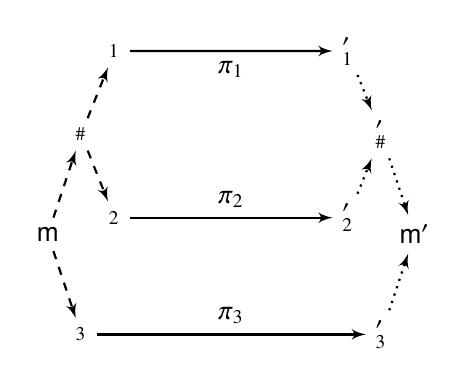
\begin{tikzpicture}[>=latex', join=bevel, initial text = , every node/.style=, scale=1.2]
  % States
  \node (m) at (0bp, 0bp) {$\modl$};

  \node (a3) at (10bp, -30bp) {$\modla_3$};
  \node (msharp) at (10bp, 30bp) {$\modla_\#$};

  \node (a3prime) at (100bp, -30bp) {$\modla'_3$};
  \node (a2) at (20bp, 5bp) {$\modla_2$};  
  \node (a1) at (20bp, 55bp) {$\modla_1$};  

  \node (msharpprime) at (100bp, 30bp) {$\modla'_\#$};
  \node (a2prime) at (90bp, 5bp) {$\modla'_2$};  
  \node (a1prime) at (90bp, 55bp) {$\modla'_1$};  

  \node (mprime) at (110bp, 0bp) {$\modl'$};
  % Edges
  % \draw[->] (0) to node [above] {$-1$} (1);
  \draw[thick, dashed, ->] (m) to node [] {} (a3);
  \draw[thick, dashed, ->] (m) to node [] {} (msharp);

  \draw[thick, dashed, ->] (msharp) to node [] {} (a2);
  \draw[thick, dashed, ->] (msharp) to node [] {} (a1);

  \draw[thick, ->] (a3) to node [above] {$\pi_3$} (a3prime);  
  \draw[thick, ->] (a2) to node [above] {$\pi_2$} (a2prime);  
  \draw[thick, ->] (a1) to node [below] {$\pi_1$} (a1prime);  

  \draw[thick, dotted, ->] (a2prime) to node [] {} (msharpprime);
  \draw[thick, dotted, ->] (a1prime) to node [] {} (msharpprime);

  \draw[thick, dotted, ->] (a3prime) to node [] {} (mprime);  
  \draw[thick, dotted, ->] (msharpprime) to node [] {} (mprime);  
  
  % Selfloops
  % \draw (0) edge [loop above] node [above] {$+1$} (0);
\end{tikzpicture}

    \end{tabular}
    \caption{\label{fig:illustration-associativity} Illustration of associativity. Visual aid for the proof of Proposition~\ref{prop:associativity}.}
  \end{figure}
  
%% \begin{figure}[h]
%% \begin{verbatim}
%%     exist m1, m*, m2, m3, m'1, m'2, m'3, m'*:

%%        m1-----------pi1-----------m'1
%%       /                             \
%%    m /                               \ m'
%%      \                               /
%%       \     m2-----pi2-----m'2      /
%%        \   /                  \    /
%%         m*/                    \m'*
%%           \                    /
%%            \                  /
%%             m3-----pi3-----m'3


%%     iff exist a#, a3, a1, a2, a'1, a'2, a'#, a'3:

%%             a1-----pi1-----a'1
%%            /                  \
%%         a#/                    \a'#
%%        /  \                    /  \
%%       /    \                  /    \
%%    m /      a2-----pi2-----a'2      \ m'
%%      \                              /
%%       \                            /
%%        a3-----------pi3-----------a'3

%% \end{verbatim}
%% \caption{\label{fig:illustration-associativity-ascii} Illustration of associativity. Visual aid for the proof of Proposition~\ref{prop:associativity}.}
%% \end{figure}

Figure~\ref{fig:illustration-associativity} illustrates precisely what we are going to show.
  %
Suppose $\modl = \tuple{\readset, \writeset, \valuset}$ and $\modl' = \tuple{\readset', \writeset', \valuset'}$.




\paragraph{Left-hand side.} $\modl \intPgm{ \pi_1 \pll (\pi_2 \pll \pi_3) } \modl'$.

There are $\modl_1, \modl_*, \modl'_1, \modl'_*$ such that (with, $\modl_1 = \tuple{\readset_1, \writeset_1, \valuset_1}$, $\modl'_1 = \tuple{\readset'_1, \writeset'_1, \valuset'_1}$, $\modl_* = \tuple{\readset_*, \writeset_*, \valuset_*}$, $\modl'_* = \tuple{\readset'_*, \writeset'_*, \valuset'_*}$):
\begin{enumerate}
\item\label{i:split-merge1}\label{i:lhsfirst} $\splt{\modl}{\modl_1} {\modl_*}$
  and $\mrg{\modl'}{\modl'_1} {\modl'_*}$ 
\item $\modl_1 \intPgm{ \pi_1 } \modl'_1$
\item $\readset_1 = \readset'_1$
  and $\writeset_1 = \writeset'_1$
  and $\valuset_1 \setminus \writeset_1 = \valuset'_1 \setminus \writeset'_1$
\item\label{i:pi2pi3} $\modl_* \intPgm{ \pi_2 \pll \pi_3 } \modl'_*$ 
\item $\readset_* = \readset'_*$
  and $\writeset_* = \writeset'_*$ 
  and $\valuset_* \setminus \writeset_* = \valuset'_* \setminus \writeset'_*$
\end{enumerate}
Item~\ref{i:pi2pi3} is equivalent to: there are $\modl_2, \modl_3, \modl'_2, \modl'_3$ such that  (with $\modl_2 = \tuple{\readset_2, \writeset_2, \valuset_2}$, $\modl'_2 = \tuple{\readset'_2, \writeset'_2, \valuset'_2}$, $\modl_3 = \tuple{\readset_3, \writeset_3, \valuset_3}$, $\modl'_3 = \tuple{\readset'_3, \writeset'_3, \valuset'_3}$):
\begin{enumerate}[resume]
\item\label{i:split-merge2} $\splt{\modl_*}{\modl_2} {\modl_3} $ and $\mrg{\modl_*'}{\modl'_2} {\modl'_3} $,
\item $\modl_2 \intPgm{ \pi_2 } \modl'_2$, 
\item $\readset_2 = \readset'_2 $ and $\writeset_2 = \writeset'_2 $ and $\valuset_2 \setminus \writeset_2 = \valuset'_2 \setminus \writeset'_2$,
\item $\modl_3 \intPgm{ \pi_3 } \modl'_3$, 
\item $\readset_3 = \readset'_3 $ and $\writeset_3 = \writeset'_3 $ and $\valuset_3 \setminus \writeset_3 = \valuset'_3 \setminus \writeset'_3$.
\end{enumerate}
Item~\ref{i:split-merge1} is $\splt{\modl}{\modl_1} {\modl_*} $ and $\mrg{\modl'}{\modl'_1} {\modl'_*} $ iff:
\begin{enumerate}[resume]
\item
  %%%% split
  $\writeset_1 \cap \readset_* = \writeset_* \cap \readset_1 = \emptyset$ ($\modl_1$ and $\modl_*$ are RW-compatible),
  \item 
    $\readset = \readset_1 \cup \readset_* $, and $\writeset = \writeset_1 \cup \writeset_*$, and $\valuset = \valuset_1 = \valuset_*$,

    %%%% merge
    
    \item $\writeset'_1 \cap \readset'_* = \writeset'_* \cap \readset'_1 = \emptyset$ ($\modl'_1$ and $\modl'_*$ are RW-compatible),
    \item $\readset' = \readset'_1 \cup \readset'_*$, $\writeset' = \writeset'_1 \cup \writeset'_*$, and $\valuset'_1 \setminus \writeset' = \valuset'_* \setminus \writeset'$, and $\valuset' = (\valuset'_1 \cap \writeset'_1) \cup (\valuset'_* \cap \writeset'_*) \cup (\valuset'_1 \cap \valuset'_*) $. 
\end{enumerate}
Item~\ref{i:split-merge2} is $\splt{\modl}{\modl_2} {\modl_3} $ and $\mrg{\modl'}{\modl'_2} {\modl'_3} $ iff:
\begin{enumerate}[resume]
\item
  %%%% split
  $\writeset_2 \cap \readset_3 = \writeset_3 \cap \readset_2 = \emptyset$ ($\modl_2$ and $\modl_3$ are RW-compatible),
  \item 
    $\readset_* = \readset_2 \cup \readset_3 $, and $\writeset_* = \writeset_2 \cup \writeset_3$, and $\valuset_* = \valuset_2 = \valuset_3$,

    %%%% merge
    
    \item $\writeset'_2 \cap \readset'_3 = \writeset'_3 \cap \readset'_2 = \emptyset$ ($\modl'_2$ and $\modl'_3$ are RW-compatible),
    \item\label{i:lhslast} $\readset_*' = \readset'_2 \cup \readset'_3$, $\writeset_*' = \writeset'_2 \cup \writeset'_3$, and $\valuset'_2 \setminus \writeset_*' = \valuset'_3 \setminus \writeset_*'$, and $\valuset_*' = (\valuset'_2 \cap \writeset'_2) \cup (\valuset'_3 \cap \writeset'_3) \cup (\valuset'_2 \cap \valuset'_3) $. 
\end{enumerate}


\paragraph{Right-hand side.} $\modl \intPgm{ (\pi_1 \pll \pi_2) \pll \pi_3 } \modl'$.

There are $\modla_\#, \modla_3, \modla_\#', \modla_3'$ such that
(with, $\modla_\# = \tuple{\readseta_\#, \writeseta_\#, \valuseta_\#}$, $\modla'_\# = \tuple{\readseta'_\#, \writeseta'_\#, \valuseta'_\#}$, $\modla_3 = \tuple{\readseta_3, \writeseta_3, \valuseta_3}$, $\modla'_3 = \tuple{\readseta'_3, \writeseta'_3, \valuseta'_3}$):
\begin{enumerate}[resume]
\item\label{i:split-merge3}\label{i:rhsfirst} $\splt{\modl}{\modla_\#} {\modla_3}$
  and $\mrg{\modl'}{\modla'_\#} {\modla'_3}$, 
\item\label{i:pi1pi2} $\modla_\# \intPgm{ \pi_1 \pll \pi_2} \modla'_\#$,
\item $\readseta_\# = \readseta'_\#$
  and $\writeseta_\# = \writeseta'_\#$
  and $\valuseta_\# \setminus \writeseta_\# = \valuseta'_\# \setminus \writeseta'_\#$,
\item $\modla_3 \intPgm{ \pi_3 } \modla'_3$, 
\item $\readseta_3 = \readseta'_3$
  and $\writeseta_3 = \writeseta'_3$ 
  and $\valuseta_3 \setminus \writeseta_3 = \valuseta'_3 \setminus \writeseta'_3$.
\end{enumerate}
Item~\ref{i:pi1pi2} is equivalent to:
there are $\modla_1, \modla_2, \modla'_1, \modla'_2$ such that 
(with, $\modla_1 = \tuple{\readseta_1, \writeseta_1, \valuseta_1}$, $\modla'_1 = \tuple{\readseta'_1, \writeseta'_1, \valuseta'_1}$, $\modla_2 = \tuple{\readseta_2, \writeseta_2, \valuseta_2}$, $\modla'_2 = \tuple{\readseta'_2, \writeseta'_2, \valuseta'_2}$):
\begin{enumerate}[resume]
\item\label{i:split-merge4} $\splt{\modla_\#}{\modla_1} {\modla_2}$
  and $\mrg{\modla'_\#}{\modla'_1} {\modla'_2}$, 
\item $\modla_1 \intPgm{ \pi_1} \modla'_1$,
\item $\readseta_1 = \readseta'_1$,
  and $\writeseta_1 = \writeseta'_1$
  and $\valuseta_1 \setminus \writeseta_1 = \valuseta'_1 \setminus \writeseta'_1$,
\item $\modla_2 \intPgm{ \pi_2 } \modla'_2$, 
\item $\readseta_2 = \readseta'_2$
  and $\writeseta_2 = \writeseta'_2$ 
  and $\valuseta_2 \setminus \writeseta_2 = \valuseta'_2 \setminus \writeseta'_2$.
\end{enumerate}
Item~\ref{i:split-merge3} is $\splt{\modl}{\modla_\#} {\modla_3}$ and $\mrg{\modl'}{\modla'_\#} {\modla'_3}$ iff:
\begin{enumerate}[resume]
\item
  %%%% split
  $\writeseta_\# \cap \readseta_3 = \writeseta_3 \cap \readseta_\# = \emptyset$ ($\modla_\#$ and $\modla_3$ are RW-compatible),
  \item 
    $\readset = \readseta_\# \cup \readseta_3 $, and $\writeset = \writeseta_\# \cup \writeseta_3$, and $\valuset = \valuseta_\# = \valuseta_3$,

    %%%% merge
    
    \item $\writeseta'_\# \cap \readseta'_3 = \writeseta'_3 \cap \readseta'_\# = \emptyset$ ($\modla'_\#$ and $\modla'_3$ are RW-compatible),
    \item $\readset' = \readseta'_\# \cup \readseta'_3$, $\writeset' = \writeseta'_\# \cup \writeseta'_3$, and $\valuseta'_\# \setminus \writeset' = \valuseta'_3 \setminus \writeset'$, and $\valuset' = (\valuseta'_\# \cap \writeseta'_\#) \cup (\valuseta'_3 \cap \writeseta'_3) \cup (\valuseta'_\# \cap \valuseta'_3) $. 
\end{enumerate}
Item~\ref{i:split-merge4} is $\splt{\modla_\#}{\modla_1} {\modla_2}$ and $\mrg{\modla'_\#}{\modla'_1} {\modla'_2}$ iff:
\begin{enumerate}[resume]
\item
  %%%% split
  $\writeseta_1 \cap \readseta_2 = \writeseta_2 \cap \readseta_1 = \emptyset$ ($\modla_1$ and $\modla_2$ are RW-compatible),
  \item 
    $\readseta_\# = \readseta_1 \cup \readseta_2 $, and $\writeseta_\# = \writeseta_1 \cup \writeseta_2$, and $\valuseta_\# = \valuseta_1 = \valuseta_2$,

    %%%% merge
    
    \item $\writeseta'_1 \cap \readseta'_2 = \writeseta'_2 \cap \readseta'_1 = \emptyset$ ($\modla'_1$ and $\modla'_2$ are RW-compatible),
    \item\label{i:rhslast} $\readseta_\#' = \readseta'_1 \cup \readseta'_2$, $\writeseta_\#' = \writeseta'_1 \cup \writeseta'_2$, and $\valuseta'_1 \setminus \writeseta_\#' = \valuseta'_2 \setminus \writeseta_\#'$, and $\valuseta_\#' = (\valuseta'_1 \cap \writeseta'_1) \cup (\valuseta'_2 \cap \writeseta'_2) \cup (\valuseta'_1 \cap \valuseta'_2) $. 
\end{enumerate}


\paragraph{Left to right.}

Suppose lhs. We define:
\begin{itemize} 
\item $\modla_\# = \tuple{\readseta_\#, \writeseta_\#, \valuseta_\#} = \tuple{\readset_1 \cup \readset_2, \writeset_1 \cup \writeset_2, \valuset}$,
\item $\modla_1 = \tuple{\readseta_1, \writeseta_1, \valuseta_1} = \modl_1 = \tuple{\readset_1, \writeset_1, \valuset}$,
\item $\modla_2 = \tuple{\readseta_2, \writeseta_2, \valuseta_2} = \modl_2 = \tuple{\readset_2, \writeset_2, \valuset}$,
\item $\modla_3 = \tuple{\readseta_3, \writeseta_3, \valuseta_3} = \modl_3 = \tuple{\readset_3, \writeset_3, \valuset}$,
\item $\modla'_\# = \tuple{\readseta'_\#, \writeseta'_\#, \valuseta'_\#} = \tuple{\readset'_1 \cup \readset'_2, \writeset'_1 \cup \writeset'_2, (\valuset'_1 \cap \writeset_1) \cup (\valuset'_2 \cap \writeset_2) \cup (\valuset'_1 \cap \valuset'_2)}$,
\item $\modla'_1 = \tuple{\readseta'_1, \writeseta'_1, \valuseta'_1) = \modl'_1 = (\readset'_1, \writeset'_1, \valuset'_1}$,
\item $\modla'_2 = \tuple{\readseta'_2, \writeseta'_2, \valuseta'_2} = \modl'_2 = \tuple{\readset'_2, \writeset'_2, \valuset'_2}$,
\item $\modla'_3 = \tuple{\readseta'_3, \writeseta'_3, \valuseta'_3} = \modl'_3 = \tuple{\readset'_3, \writeset'_3, \valuset'_3}$. 
\end{itemize}

We must show that these models satisfy all the properties from~\ref{i:rhsfirst} through~\ref{i:rhslast}.
\begin{itemize}
\item[19] if and only if
  \begin{itemize}
  \item[29]  $\writeseta_\# \cap \readseta_3 = \emptyset$,
    $\writeseta_3 \cap \readseta_\# = \emptyset$. It holds because:
    \begin{itemize}
    \item $\writeseta_\# \cap \readseta_3 = (\writeset_1 \cup \writeset_2) \cap \readset_3 = (\writeset_1 \cap \readset_3) \cup (\writeset_2 \cap \readset_3)$.
      By 15, we have $\writeset_2 \cap \readset_3 = \emptyset$.
      By 16, we have $\readset_3 \subseteq \readset_*$.
      By 11, we have $\writeset_1 \cap \readset_* = \emptyset$. So, $\writeset_1 \cap \readset_3 = \emptyset$.
    \item $\writeseta_3 \cap \readseta_\# = \writeset_3 \cap (\readset_1 \cup \readset_2) = (\writeset_3 \cap \readset_1) \cup (\writeset_3 \cap \readset_2)$.
      By 15, we have $\writeset_3 \cap \readset_2 = \emptyset$.
      By 11, we have $\writeset_* \cap \readset_1 = \emptyset$.
      By 16, we have $\writeset_3 \subseteq \writeset_*$.
      So, $\writeset_3 \cap \readset_1 = \emptyset$.
    \end{itemize}
  
  \item[30]
    %$\readset = \readseta_\# \cup \readseta_3$?
$\readseta_\# \cup \readseta_3 = (\readset_1 \cup \readset_2) \cup \readset_3 = \readset_1 \cup \readset_* = \readset$ (definition and 16 and 12).
    % $\writeset = \writeseta_\# \cup \writeseta_3$?
    $\writeseta_\# \cup \writeseta_3 = (\writeset_1 \cup \writeset_2) \cup \writeset_3 = \writeset_1 \cup \writeset_* = \writeset$ (definition and 16 and 12).
    % $\valuset = \valuseta_\# = \valuseta_3$?
    $\valuset = \valuseta_\# = \valuseta_3$ (definition).
    
  \item[31] $\writeseta'_\# \cap \readseta'_3 = \writeseta'_3 \cap \readseta'_\# = \emptyset$. It holds because:
    \begin{itemize}
    \item $\writeseta'_\# \cap \readseta'_3 = (\writeset'_1 \cup \writeset'_2) \cap \readset'_3$ by definition. It is equal to $(\writeset_1 \cap \readset_3) \cup (\writeset_2 \cap \readset_3)$, by 3, 8, 10. We have $\writeset_1 \cap \readset_* = \emptyset$ (11), and $\readset_3 \subset \readset_*$ (16). So $\writeset_1 \cap \readset_3 = \emptyset$.
      We have $\writeset_2 \cap \readset_3 = \emptyset$ (15).
    \item $\writeseta'_3 \cap \readseta'_\# = \writeseta'_3 \cap (\readset'_1 \cup \readset'_2)$ by definition. It is equal to $(\writeseta_3 \cap \readset_1) \cup (\writeseta_3 \cap \readset_2)$, by 10, 3, 8. We have $\writeset_3 \subseteq \writeset_*$ (16) and $\writeset_* \cap \readset_1 = \emptyset$ (11).
      So $\writeseta_3 \cap \readset_1 = \emptyset$.
      We have $\writeseta_3 \cap \readset_2 = \emptyset$ (15).
    \end{itemize}

  \item[32]
    \begin{itemize}
    \item Instrumental claims:
      \begin{itemize}
  \item(claim~1) $\writeset'_* = \writeset_*$, by 16, 7, 9 and 18.
  \item(claim~2) $\writeset = \writeset'$, by 12, 3, claim~1, 14.
  \item(claim~3) $\writeset_1 \subseteq \writeset'$, by claim~2, and 12.
  \item(claim~4.1) $\writeset_2 \subseteq \writeset'$, by claim~2, 16, and 12.
  \item(claim~4.2) $\writeset_3 \subseteq \writeset'$, by claim~2, 16, and 12.    
  \item(claim~5) $\valuset'_1 \setminus \writeset' = \valuset_1 \setminus \writeset'$, by 3, 12, and claim~2.
  \item(claim~6) $\valuset'_2 \setminus \writeset' = \valuset_2 \setminus \writeset'$, by 8, 16, and 12.
  \item(claim~7) $\valuset'_3 \setminus \writeset' = \valuset_3 \setminus \writeset'$, by 10, 16, and 12.
  \item(claim~8) $\writeset_1 \cap \writeset_2 = \emptyset$, by 11, 12, the `write-set included in read-set' model constraint, and 16.
      \end{itemize}
    \item $\readset' = \readseta'_\# \cup \readseta'_3$ and $\writeset' = \writeseta'_\# \cup \writeseta'_3$ hold by definition, 16 and 12. 

    \item $\valuseta'_\# \setminus \writeset' = \valuseta'_3 \setminus \writeset'$ holds because:
      \begin{itemize}
        \item $\valuseta'_\# \setminus \writeset' = (\valuset_1' \cup \valuset_2') \setminus \writeset'$ by definitions, claim~3, and claim~4.1. By claim~5 and claim~6, it is equal to $(\valuset_1 \cup \valuset_2) \setminus \writeset'$, which by 12 and 16 is $\valuset \setminus \writeset'$.
          %
          \item
      Moreover, $\valuseta'_3 \setminus \writeset' = \valuset'_3 \setminus \writeset'$ by definition. It is equal to $\valuset_3 \setminus \writeset'$ by claim~7, and to $\valuset \setminus \writeset'$ by 12 and 16.
      \end{itemize}
    \item $\valuset' = (\valuseta'_\# \cap \writeseta'_\#) \cup (\valuseta'_3 \cap \writeseta'_3) \cup (\valuseta'_\# \cap \valuseta'_3)$  holds because:
      \begin{itemize}
      \item $\valuseta'_\# \cap \writeseta'_\# = ((\valuset'_1 \cap \writeset'_1) \cup (\valuset'_2 \cap \writeset'_2) \cup (\valuset'_1 \cap \valuset'_2)) \cap (\writeset'_1 \cup \writeset'_2)$ by definition, 3, and 8. We get $(\valuset'_1 \cap \writeset'_1 \cap \writeset'_1) \cup (\valuset'_1 \cap \writeset'_1 \cap \writeset'_2) \cup (\valuset'_2 \cap \writeset'_2 \cap \writeset'_1) \cup (\valuset'_2 \cap \writeset'_2 \cap \writeset'_2) \cup (\valuset'_1 \cap \valuset'_2 \cap \writeset'_1) \cup (\valuset'_1 \cap \valuset'_2 \cap \writeset'_2)$. With elementary set theory simplifications and claim~8, we obtain $(\valuset'_1 \cap \writeset'_1) \cup (\valuset'_2 \cap \writeset'_2)$.
\item $\valuseta'_3 \cap \writeseta'_3 = \valuset'_3 \cap \writeset'_3$.
\item $\valuseta'_\# \cap \valuseta'_3 ((\valuset'_1 \cap \writeset'_1) \cup (\valuset'_2 \cap \writeset'_2) \cup (\valuset'_1 \cap \valuset'_2)) \cap \valuset'_3$ by definition, 3, and 8. We get $(\valuset'_1 \cap \writeset'_1 \cap \valuset'_3) \cup (\valuset'_2 \cap \writeset'_2 \cap \valuset'_3) \cup (\valuset'_1 \cap \valuset'_2 \cap \valuset'_3)$.
\item The rhs quantity $(\valuseta'_\# \cap \writeseta'_\#) \cup (\valuseta'_3 \cap \writeseta'_3) \cup (\valuseta'_\# \cap \valuseta'_3)$ is then equal to
  $(\valuset'_1 \cap \writeset'_1) \cup (\valuset'_2 \cap \writeset'_2) \cup
  (\valuset'_3 \cap \writeset'_3) \cup (\valuset'_1 \cap \valuset'_2 \cap \valuset'_3)$.
\item Moreover, by 14, we have $\valuset' = (\valuset'_1 \cap \writeset'_1) \cup (\valuset'_* \cap \writeset'_*) \cup (\valuset'_1 \cap \valuset'_*)$.
\item By 18, $\valuset'_* = (\valuset'_2 \cap \writeset'_2) \cup (\valuset'_3 \cap \writeset'_3) \cup (\valuset'_1 \cap \valuset'_2)$.
\item By claim~1, $\writeset'_* = \writeset_*$, which by 16 is $\writeset_2 \cup \writeset_3$ which by 8 and 10 is $\writeset'_2 \cup \writeset'_3$. So $\writeset'_2 \subseteq \writeset'_*$ and $\writeset'_3 \subseteq \writeset'_*$.
\item So $(\valuset'_* \cap \writeset'_*) = (\valuset'_2 \cap \writeset'_2) \cup (\valuset'_3 \cap \writeset'_3) \cup (\valuset'_1 \cap \valuset'_2 \cap \writeset'_*)$, with $\valuset'_1 \cap \valuset'_2 \cap \writeset'_* = \valuset'_1 \cap \valuset'_2 \cap (\writeset'_2 \cup \writeset'_3)$ by 18, which is $(\valuset'_2 \cap \valuset'_3 \cap \writeset'_2) \cup (\valuset'_2 \cap \valuset'_3 \cap \writeset'_3)$. So $(\valuset'_* \cap \writeset'_*) = (\valuset'_2 \cap \writeset'_2) \cup (\valuset'_3 \cap \writeset'_3)$.
\item Also $(\valuset'_1 \cap \valuset'_*) = (\valuset'_1 \cap \valuset'_2 \cap \writeset'_2) \cup (\valuset'_1 \cap \valuset'_3 \cap \writeset'_3) \cup (\valuset'_1 \cap \valuset'_2 \cap \valuset'_3)$, with the first two disjuncts included in $\valuset'_* \cap \writeset'_*$.
\item The lhs quantity $V'$ is then equal to $(\valuset'_1 \cap \writeset'_1) \cup (\valuset'_2 \cap \writeset'_2) \cup
  (\valuset'_3 \cap \writeset'_3) \cup (\valuset'_1 \cap \valuset'_2 \cap \valuset'_3)$.
      \end{itemize}
    \end{itemize}

  \end{itemize}


\item[20] if and only if

  \begin{itemize}
  \item[24] if and only if
  \begin{itemize}
  \item[33] $\writeseta_1 \cap \readseta_2 = \emptyset$,
    $\writeseta_2 \cap \readseta_1 = \emptyset$. It holds, because:
    \begin{itemize}

    \item $\writeseta_1 \cap \readseta_2 = \writeset_1 \cap \readset_2$ by definition.
    From 16, $\readset_2 \subseteq \readset_*$. From 11, $\writeset_1 \cap \readset_* = \emptyset$. So $\writeset_1 \cap \readset_2 = \emptyset$.

    \item $\writeseta_2 \cap \readseta_1 = \writeset_2 \cap \readset_1$ by definition.
    From 16, $\writeset_2 \subseteq \writeset_*$. From 11, $\writeset_* \cap \readset_1 = \emptyset$. So $\writeset_2 \cap \readset_1 = \emptyset$.
    \end{itemize}
  \item[34] By definition.
  \item[35] By definition, 33, 3, and 8.
  \item[36] $\readseta_\#' = \readseta'_1 \cup \readseta'_2$, $\writeseta_\#' = \writeseta'_1 \cup \writeseta'_2$, and $\valuseta_\#' = (\valuseta'_1 \cap \writeseta'_1) \cup (\valuseta'_2 \cap \writeseta'_2) \cup (\valuseta'_1 \cap \valuseta'_2)$ by definition.
%
    Also, $\valuseta'_1 \setminus \writeseta_\#' = \valuseta'_2 \setminus \writeseta_\#'$ holds because:
    \begin{itemize}
    \item $\valuseta'_1 \setminus \writeseta_\#' = \valuset'_1 \setminus (\writeset'_1 \cup \writeset'_2)$, which by 3 and 8 is equal to $\valuset_1 \setminus (\writeset_1 \cup \writeset_2)$, which by 12 is equal to $\valuset \setminus (\writeset_1 \cup \writeset_2)$.
      \item Similarly, $\valuseta'_2 \setminus \writeseta_\#'$ is equal to $\valuset \setminus (\writeset_1 \cup \writeset_2)$ by 8, 3, 16 and 12.
    \end{itemize}
  \end{itemize}
\item[25] By definition, and 2.
\item[26] By definition, 3, and 12.
\item[27] By definition, and 7.
\item[28] By definition, 8, 16, and 12.
  \end{itemize}
\item[21] $\readseta_\# = \readseta'_\#$
  and $\writeseta_\# = \writeseta'_\#$ hold by definition, 3, and 8.
  Also by definition, 3, and 8, $\valuseta_\# \setminus \writeseta_\# = \valuseta'_\# \setminus \writeseta'_\#$ is equivalent to $\valuset \setminus (\writeset_1 \cup \writeset_2) = ((\valuset'_1 \cap \writeset'_1) \cup (\valuset'_2 \cap \writeset'_2) \cup (\valuset'_1 \cap \valuset'_2)) \setminus (\writeset_1 \cup \writeset_2)$. The right-hand-side simplifies into $(\valuset'_1 \cap \valuset'_2) \setminus (\writeset_1 \cup \writeset_2)$. Moreover, we have $\valuset'_1 \setminus \writeset'_1 = \valuset \setminus \writeset'_1$ (by 3 and 12) and $\valuset'_2 \setminus \writeset'_2 = \valuset \setminus \writeset'_2$ (by 8, 16, and 12). So we have $\valuset'_1 \setminus (\writeset'_1 \cup \writeset'_2) = \valuset \setminus (\writeset'_1 \cup \writeset'_2)$ and $\valuset'_2 \setminus (\writeset'_1 \cup \writeset'_2) = \valuset \setminus (\writeset'_1 \cup \writeset'_2)$. Hence, $(\valuset'_1 \cap \valuset'_2) \setminus (\writeset_1 \cup \writeset_2)$ simplifies into the left-hand-side $\valuset \setminus (\writeset_1 \cup \writeset_2)$.
\item[22] By definition, and 9.
\item[23] By definition, 10, 16, and 12.
\end{itemize}


\paragraph{Right to left.}

Suppose rhs. We define:
\begin{itemize}
\item $\modl_* = \tuple{\readset_*, \writeset_*, \valuset_*} = \tuple{\readseta_2 \cup \readseta_3, \writeseta_2 \cup \writeseta_3, \valuset}$,

\item $\modl_1 = \tuple{\readset_1, \writeset_1, \valuset_1} = \modla_1 = \tuple{\readseta_1, \writeseta_1, \valuseta}$,
\item $\modl_2 = \tuple{\readset_2, \writeset_2, \valuset_2} = \modla_2 = \tuple{\readseta_2, \writeseta_2, \valuseta}$,
\item $\modl_3 = \tuple{\readset_3, \writeset_3, \valuset_3} = \modla_3 = \tuple{\readseta_3, \writeseta_3, \valuseta}$,  

\item $\modl'_* = \tuple{\readset'_*, \writeset'_*, \valuset'_*} = \tuple{\readseta'_2 \cup \readseta'_3, \writeseta'_2 \cup \writeseta'_3, (\valuseta'_2 \cap \writeseta_2) \cup (\valuseta'_3 \cap \writeseta_3) \cup (\valuseta'_2 \cap \valuseta'_3)}$,
  
\item $\modl'_1 = \tuple{\readset'_1, \writeset'_1, \valuset'_1} = \modla'_1 = \tuple{\readseta'_1, \writeseta'_1, \valuseta'_1}$,
\item $\modl'_2 = \tuple{\readset'_2, \writeset'_2, \valuset'_2} = \modla'_2 = \tuple{\readseta'_2, \writeseta'_2, \valuseta'_2}$,
\item $\modl'_3 = \tuple{\readset'_3, \writeset'_3, \valuset'_3} = \modla'_3 = \tuple{\readseta'_3, \writeseta'_3, \valuseta'_3}$. 
\end{itemize}

We must show that these models satisfy all the properties from~\ref{i:lhsfirst} to~\ref{i:lhslast}. This is done routinely, analogously to the proof of the left-to-right direction above.
\end{proof}

%%% Local Variables:
%%% mode: latex
%%% TeX-master: "x_dlpa4para.tex"
%%% End:


%\bibliographystyle{plainurl}
\bibliographystyle{alpha}
\bibliography{biblio}

\end{document}
